\documentclass[11pt]{book}
\frenchspacing
\usepackage{geometry}

\usepackage[parfill]{parskip}
\usepackage{graphicx}
\usepackage{amssymb}
\usepackage{epstopdf}
\DeclareGraphicsRule{.tif}{png}{.png}{ 'convert #1 ' dirname #1' /' basename #1 .tif' .png}

\usepackage[T1]{fontenc}
\usepackage{textcomp}

%% LaTeX - Article customise

%%% PACKAGES
\usepackage{booktabs} % for much better looking tables
\usepackage{array} % for better arrays (eg matrices) in maths
\usepackage{verbatim} % adds environment for commenting out blocks of text & for better verbatim
\usepackage{amsmath}

\usepackage[svgnames]{xcolor}
\usepackage{listings}
\lstdefinelanguage{kappa}{
	alsoletter={\%,:,-,<,>,@},
	morekeywords=[1]{\%agent\:, \%token\:, \%var\:, \%obs\:},
	morekeywords=[2]{\%init\:},
	morekeywords=[3]{\%mod\:, \%def\:, \$ADD, \$DEL, \$SNAPSHOT, \$STOP, \$FLUX, \$TRACK, \$UPDATE, \$PLOTENTRY, \$PRINT, \$PRINTF},
	morekeywords=[4]{->, <->, @},
	morestring=[d]{'},
	morecomment=[l]\#
}
\lstset{	
	basicstyle=\ttfamily,
	numbers=left,
	numberstyle=\tiny,
	breaklines,
	keywordstyle=[1]\color{LightSlateBlue},
	keywordstyle=[2]\color{Brown},
	keywordstyle=[3]\color{DarkOrange},
	keywordstyle=[4]\color{Red},
	stringstyle=\color{ForestGreen},
	commentstyle=\color{LightSlateGrey}
}
\renewcommand{\lstlistlistingname}{Codes}
\renewcommand{\lstlistingname}{Code}

\usepackage[linktoc=page,colorlinks=true]{hyperref}
\expandafter\let\csname NR:Type\endcsname\relax

\usepackage{makeidx}
\usepackage{color}

\def\KaSimLogo{img/KaSim-Logo.pdf}

\usepackage{fancyhdr} %to insert logo on the left head of each page
\pagestyle{fancy}
\begin{titlepage}
\rhead{\includegraphics[width=35mm,natwidth=375pt,natheight=200pt]{\KaSimLogo}}
\end{titlepage}

\def\KaSim{\textsf{KaSim}}
\def\KaSa{\textsf{KaSa}}
\def\sep{\hbox{-}}
\def\int{\textasciitilde}
\def\intstate{\textasciitilde}
\def\tcb#1{\textcolor{blue}{\ttt{#1}}}
\def\ttt#1{\texttt{#1}}
\def\var#1{{\textquotesingle}#1{\textquotesingle}}

\makeindex

%% END Article customise

%%%% added by Vincent to compensate for the lack of mystyle.sty
\frenchspacing
\def\rar{\rightarrow}
\def\lrar{\leftrightarrow}

\def\ka{\kappa}
\def\ga{\gamma}
\def\bs{\backslash}
\def\noi{\noindent}
\def\ie{ie }
\def\via{via }
\def\set#1{\{#1\}}
\def\ITE#1{\begin{itemize}#1\end{itemize}}
\def\ENU#1{\begin{enumerate}#1\end{enumerate}}
\def\mit#1{{\mathit #1}}
\def\Real{\mathbb R}
\def\Nat{\mathbb N}
\def\Z{\mathbb Z}
\def\dd{-\hspace{0.001cm}-}
\def\imp#1{\emph{#1}\index{#1}}
%%%%

\newcommand{\Remark}{\paragraph{Remark}}

\def\version{3.90}

\title{KaSim~\& KaSa~reference manual\\ \small (release \version)}
\author{Pierre Boutillier, J\'er\^ome Feret, Jean Krivine\thanks{corresponding author: jean.krivine@pps.univ-paris-diderot.fr} and L\'y Kim Quy\^en \\\href{http://www.kappalanguage.org}{KappaLanguage.org}}

\date{}
                                    % Activate to display a given date or no date
\begin{document}
\maketitle

%\begin{center}\includegraphics[width=80mm]{img/wip.jpg}
%\vspace{3cm}
%\\This document is work in progress...
%\end{center}

\tableofcontents
\listoftables

\chapter{Introduction}
\begin{center}\includegraphics[width=9cm,natwidth=375pt,natheight=200pt]{\KaSimLogo}\end{center}

\section{Preamble}
This manual describes the usage of \KaSim~and \KaSa, the latest implementation of Kappa, one member of the growing family of rule-based languages. Rule-based modelling has attracted recent attention in developing biological models that are concise, comprehensible, easily extensible, and allows one to deal with the combinatorial complexity of multi-state and multi-component biological molecules.
Although this manual contains a self-contained description of Kappa, it is \emph{not} intended as a tutorial on rule-based modeling.%%Therefore, in the following of this manual some familiarity with Kappa is assumed and
%

To get an idea of how Kappa is used in a modeling context, the reader can consult the following note \href{http://www.pps.univ-paris-diderot.fr/~danos/pdf/eov.pdf}{Agile modelling of cellular signalling (SOS'08)}. A longer article, expounding on causal analysis is also available: \href{http://www.pps.univ-paris-diderot.fr/~danos/pdf/ka-fix.pdf}{Rule-based modelling of cellular signalling (CONCUR'07)}. See also this tutorial: \href{http://www.pps.univ-paris-diderot.fr/~danos/pdf/mytdg.pdf}{Modelling epigenetic information maintenance: a Kappa tutorial (CAV'09)}.




\section{The \KaSim~engine}
\KaSim~is an open source stochastic simulator of rule-based models~\cite{DanLan04,Dan_etal07a,Fae_etal05} written in Kappa. The Kappa language describes site graphs and their local transformations. \KaSim~takes one or several \hyperref[chap:kappa]{Kappa files} as input and generates stochastic trajectories of various observables. \KaSim~implements Danos \textit{et al}'s implicit state simulation algorithm~\cite{Dan_etal07b} which adapts Gillespie's algorithm~\cite{Gil76,Gil77} to rule-based models.

A \emph{simulation event}\index{event} corresponds to the application of a rewriting rule, contained in the Kappa files, to the current graph\index{graph} (also called a \emph{mixture}\index{mixture}).
%The rule is selected according to its \emph{activity}\index{activity}, \ie the number of instances it has in the current mixture\index{mixture}, multiplied by its kinetic rate\index{kinetic rate}
At each step, the next event %(if any)
is selected with a probability which is proportional to the rate\index{rate} of the rule it is an event of.
%It is then applied to one of its possible instances in the graph.
%The result of triggerring this event is a new graph.
If there are no events, that is to say if none of the rules apply to the current state of the system, one has a \emph{deadlock}. Note that a given rule will in general apply in many different ways; one says it has many instances. The \emph{activity}\index{activity} of a rule is the number of its instances in the current mixture\index{mixture} multiplied by its rate. The probability that the next event is associated to a given rule is therefore proportional to the activity of the rule.
Rule activities\index{activity} are updated at
each step (see Fig.~\ref{fig:event-loop}). Importantly, the cost of a simulation event is bounded by a constant that is independent of the size of the graph it is applied to~\cite{Dan_etal07b}.

\begin{figure}[htbp]
\begin{center}
\includegraphics[width=14cm]{img/event-loop.png}
\caption{The event loop}
\label{fig:event-loop}
\end{center}
\end{figure}

Note that \KaSim~can only render curves in the svg format. However, data outputs given in a text format can be displayed using any standard plotting software such as \href{http://www.gnuplot.info/}{gnuplot}.

\section{The \KaSa~static analyser}

\KaSa~is an open source static analyser  tool of rule-based models~\cite{DanLan04,Dan_etal07a,Fae_etal05} written in Kappa. \KaSa~takes one or several \hyperref[chap:kappa]{Kappa files} as input and some command line options to toggle on/off some specific static analysis. Currently, \KaSa~can compute the contact map and the influence map. It can perform reachability analysis \cite{Feret-ICCMSE2007,DanosEtAl-VMCAI08} as well.  Other analyses including  model reduction \cite{Feret-et-al-pnas2009,DanosEtAl-LICS2010,Feret-MFPSXXVII} will come soon.

A graphical interface is proposed to navigate through the various options and utilities  of \KaSa. The compilation of this interface requires \href{https://forge.ocamlcore.org/projects/labltk/}{labltk} and, in particular,  \href{http://www.tcl.tk/}{tk-dev}.


\section{Support}
\ITE{
\item[-] Kappa language tutorials and downloads: \url{http://kappalanguage.org}
\item[-] Bug reports should be posted on github: \url{https://github.com/Kappa-Dev/KaSim/issues}
\item[-] Questions and answers on the kappa-user mailing list: \url{http://groups.google.com/group/kappa-users}
\item[-] Want to contribute to the project? \ttt{jean.krivine@pps.univ-paris-diderot.fr}
}

\chapter{Installation}\label{chap:install}

\section{Using precompiled binaries}
The easiest way to use \KaSim~and \KaSa~is to use pre-compiled versions available in the release section on the github repository (\url{https://github.com/Kappa-Dev/KaSim/releases}). Download the version that corresponds to your operating system (Windows, Linux or Mac OSX) and rename the downloaded file into \KaSim~and \KaSa. Note that on Mac OSX or Linux, it might be necessary to give executable permissions to \KaSim~and \KaSa. This can be done using the shell commands:
\ttt{chmod u+x KaSim} and \ttt{chmod u+x KaSa}

To test whether your program does work, simply type \ttt{./KaSim \dd version} on a terminal, from the directory that contains the binaries. If the version is displayed it means that the binaries are indeed compatible with your OS. Otherwise you may need to compile \KaSim~from the sources (see next Section).

\section{Obtaining the sources}\label{sec:sources}
To obtain \KaSim/\KaSa~you can either use pre-compiled binaries (see
previous section) or compile the sources for your
architecture by yourself.

To do so, download the source code from
\url{https://github.com/Kappa-Dev/KaSim}, make sure you have a recent
OCaml compiler (\KaSim/\KaSa~currently requires Ocaml 4.02.3 to
compile) as well as \ttt{ocamlbuild}, \ttt{findlib} and the
\ttt{yojson} library installed.

You can check if it is the case from a terminal window by typing
first \ttt{ocamlfind ocamlopt -v}. If it fails or prints a version number
too old, then you need to install Ocaml Native compiler that can be
downloaded from \url{http://caml.inria.fr/download.en.html} and/or
findlib available at
\url{http://projects.camlcity.org/projects/findlib.html}.

Then, type \ttt{ocamlfind query yojson}. The answer should be a
path. If it is not, install yojson using a package manager.

Ocamlbuild is hosted on \url{https://github.com/ocaml/ocamlbuild}.

\section{Compilation}
Once OCaml is safely installed, untar \KaSim~archive and compile following these
few steps: \ITE{
\item[\$]\ttt{tar xzvf kasim.tar.gz -d Kappa}
\item[\$]\ttt{cd Kappa}
\item[\$]\ttt{make bin/KaSim}
\item[\$]\ttt{make bin/KaSa}}

At the end of these steps you should see, in the
\ttt{bin} directory of the \ttt{Kappa} directory, an executable file named
KaSim.  In order to check the compilation went fine, simply type
\ttt{bin/KaSim -\,-version}.

If the tool \ttt{ocamlbuild} is not in your path, you may
set the variable \ttt{OCAMLBINPATH} to point to the location of the
compiler by doing \ttt{make OCAMLBINPATH='the\_correct\_dir' bin/KaSim}.

\section{Compilation of KaSa~graphical interface}

The graphical interface of \KaSa~requires
\href{http://www.tcl.tk/}{tk-dev} and
\href{https://forge.ocamlcore.org/projects/labltk/}{labltk}. By
default, the graphical interface is not compiled. The compilation of
this interface can be toggled on by using the following command:
\ttt{make USE\_TK=1 bin/KaSa}

Common compilation errors are the following:
\begin{enumerate}
\item The following error:

\begin{verbatim}
/usr/bin/ld: cannot find -ltk
collect2: error: ld returned 1 exit status
File "caml_startup", line 1:
Error: Error during linking
Command exited with code 2.
\end{verbatim}

occurs when the module  \href{http://www.tcl.tk/}{tk-dev} is not installed.
\item The following error:

\begin{verbatim}
File "_none_", line 1:
Error: Cannot find file jpflib.cmxa
Command exited with code 2.
\end{verbatim}

occurs when ocaml cannot link the labltk library.

Please document the variable \texttt{LABLTKLIBREP} in the Makefile.

\end{enumerate}

\chapter{The kappa language}\label{chap:kappa}

\section{General structure}
A model is represented in Kappa by a set of \emph{Kappa File}. We use
KF\index{kappa file} to denote the union of the files that are given
as input (to either \KaSim~or \KaSa).

Each line of the KF\index{kappa file} is interpreted as a
\emph{declaration}\index{declaration} except if the line ends by
the~{\textquotesingle} \ttt{$\bs$}{\textquotesingle}
character. Therefore, in order to write a
declaration\index{declaration} on several lines, ends every by the
last of the lines with a \ttt{$\bs$}.

Declarations can be: agent and token \emph{signatures}
(Sec.~\ref{sec:sig}), \emph{rules}\index{rule} (Sec.~\ref{sec:rules}),
\emph{variables}\index{variable} (Sec.~\ref{sec:var}), \emph{initial
  conditions}\index{initial condition} (Sec.~\ref{sec:init}),
\emph{perturbations}\index{perturbation} (Sec.~\ref{sec:mod}) and
\emph{parameter configurations} (Sec.~\ref{sec:param}).

The KF\index{kappa file}'s structure is quite flexible. Neither
dividing into several sub-files nor the order of
declaration\index{declaration}s matters (to the exception of variable
declaration\index{declaration}s, see Section~\ref{sec:var} for
details).

Comments\index{comments} can be used either by inserting the marker
\ttt{\#} that tells \KaSim~to ignore the rest of the line or by
putting any text between the delimiters \ttt{/*} and \ttt{*/}. The
combined use of \ttt{$\bs$} and \ttt{\#} is an alternative way to
write comments in the middle of a declaration\index{declaration}.

\section{Agent and token signatures}\index{agent signature}\label{sec:sig}
%
In Kappa there are two entities that can be used for representing
biological elements: \imp{agents} and \imp{tokens}.  Agents are used
to represent complex molecules that may bind to other molecules on
specific sites. Tokens are typically used to represent small particles
such as ions, ATP, etc. Tokens cannot bind to each other, they can
only appear or disappear. In a given model, agents always have a
discrete number of instances while tokens may have a continuous
concentration.

In order to use agents or tokens in a model, one needs to declare them
first. \emph{Agent signatures}\index{agent signature} constitute a
form of typing information about the agents that are used in the
model. It contains information about the name and number of
interaction sites the agent has, and about their possible internal
states. A signature\index{agent signature} is declared in the
KF\index{kappa file} by the following line: \ITE{
\item[] \ttt{\%agent: } \textit{signature\_expression} } according to
the grammar given Table~\ref{tab:sig} where terminal symbols are
written in (blue) typed font, and $\varepsilon$ stands for the empty
list. An identifier \ttt{Id} can be any string generated by a regular
expression of the type $[a\sep z\ A\sep Z][a\sep z\ A \sep Z\ 0\sep
  9\ \_ \ -\ +]^*$.
%%
\begin{table}[htbp]
  \centering
  \caption{Agent signature%\index{agent signature}
 expression}
  \begin{tabular}{@{} lcl @{}}
    \textit{signature\_expression} & ::= &
    \tcb{Id}\tcb{(}\textit{sig}\tcb{)} \\

    \textit{sig} & ::= &
    \tcb{Id}~\textit{internal\_state\_list}\tcb{,}\ \textit{sig}
    $\mid\varepsilon$ \\

    \textit{internal\_state\_list} & ::= &
    \tcb{\intstate{}Id}~\textit{internal\_state\_list}
    $\mid\varepsilon$
    \end{tabular}
  \label{tab:sig}
\end{table}
%%

For instance the line:
\begin{lstlisting}[language=kappa]
%agent: A(x,y~u~p,z~0~1~2) # Signature of agent A
\end{lstlisting}
will declare an agent \ttt{A} with 3 \emph{(interaction) sites}
\ttt{x,y} and \ttt{z} with the site \ttt{y} possessing two
\emph{internal states}\index{internal state} \ttt{u} and \ttt{p} (for
instance for the unphosphorylated and phosphorylated forms of \ttt{y})
and the site \ttt{z} having three possible states $0$, $1$ and
$2$. Note that internal states\index{internal state} values are
treated as untyped symbols by \KaSim, so choosing a character or an
integer as internal state is purely a matter of convention.

Token signature\index{agent signature}s are declared using a statement
of the form:
\begin{lstlisting}[language=kappa]
%token: ca+ # Signature of calcium token
\end{lstlisting}

\section{Sited-graph pattern: Kappa expression}

The state of the system is represented in Kappa as a sited graph: a
graph were edges specifies a site of the node they use. You must think
as sites as resources. At most one edge of the graph can use a site of
a node (representing an agent in our case). We call this concept the
\emph{rigidity of Kappa}.

\subsection{Graph syntax}
The ascii syntax we use to represent sited graphs follows the
skeletons (describe formaly in fig~\ref{tab:patterns}):
\begin{itemize}
\item we write the type of the agent and then its interface (the comma
  separeted list of the state of its sites) between parenthesis.
\item When the site is \emph{free} (is not a member of a edge) you
  just write its name to represent its state. If it has a internal
  state, you write it after a '\intstate'. For example, the graph
  TODO is written A(x,y\intstate{}p,z\intstate{}0)
\item When a site is part of an edge, you assign an integer identifier
  $n$ to this edge and you specify the appartenance of the site to
  this edge by writing site\_name$!n$. The graph TODO can be
  reprensented as A(x!23,y\intstate{}u!4,z\intstate{}1),
  A(x!4,y\intstate{}u!954,z\intstate{}1),
  A(x!95,y\intstate{}u!234,z\intstate{}1).

  \Remark{Each link identifier appears exactly twice of course. this is a
  consequence of the regidity of Kappa.}
\end{itemize}

\subsection{Pattern syntax}
Kappa strength is to describe transformations by only mentionning (and
storing) the relevant part of the subgraph required for that
transfor;ation to be possible. It plays a key role in resisting
combinatorial explosion when writing models. We use the \emph{don't
  care, don't write}\index{don't care don't write} principle. If a
transformation occurs independently of the state of a site of an
agent, don't mention it in the \emph{pattern} to match. The pattern
A(x,z) represents an agent of type A whose sites x and z are free but
the sites y and z can be in any internal state and the site y can be
linked or not to anything.

If the link state of a site does not matter but the internal state
does, an '?' has to be added after the site name (and internal state).
An agent A whose sites x and z are free, y is in state u and z in
state 2 is written A(x,y\intstate{}u?4,z\intstate{}2).

\begin{table}[ht!]
  \centering
  \caption{Kappa expressions}
  \begin{tabular}{@{} lcl @{}}
    \textit{kappa\_expression} & ::= & \textit{agent\_expression} \tcb{,} \textit{kappa\_expression} $\mid\varepsilon$ \\
    \textit{agent\_expression} & ::= &  \tcb{Id}\tcb{(}\textit{interface}\tcb{)} \\
    \textit{interface} &::=& \tcb{Id} \textit{internal\_state link\_state}  \tcb{,} \textit{interface} $\mid\varepsilon$ \\
    \textit{internal\_state} &::=& $\varepsilon$ | \tcb{\intstate Id} \\
    \textit{link\_state} &::=& $\varepsilon$ | \tcb{!n} | \tcb{!\_} | \tcb{?}  | \tcb{!Id.Id} \\
    \end{tabular}
  \label{tab:patterns}
\end{table}

\subsection{Link type}

In standard kappa, in order to require a site to be bound for an
interaction to occur, one may use the
\emph{semi-link}\index{semi-link} construct \ttt{!\_} which does not
specify who the partner of the bond is. For instance in the variable:
\lstinline[language=kappa]*%var: \var{ab}~|A(x!_),B(y!_)|* will
count the number of \ttt{A}s and \ttt{B}s connected to someone,
including the limit case \ttt{A(x!1),B(y!1)}. It is sometimes
convenient to specify the \emph{type}\index{link type} of the
semi-link, in order to restrict the choice of the binding partner. For
instance the variable:
\lstinline[language=kappa]*%var: \var{ab}~|A(x!y.B),B(y!x.A)|!*
will count the number of \ttt{A}s whose
site \ttt{x} is connected to a site \ttt{y} of \ttt{B}, plus the
number of \ttt{B}s whose site \ttt{y} is connected to a site \ttt{x}
of \ttt{A}. Note that this still includes the case
\ttt{A(x!1),B(y!1)}.

\Remark{Transformations on semi-links and links type indiuce side
  effects (effect on unmention agents/unmentionned site of agent) and
  can even don't make sense at all. What would mean to remove the link
  to A but not the link to B in the example above? Be carefull when
  you use them.}

\section{Rules}\label{sec:rules}

Once agents are declared, one may add to the KF\index{kappa file} the
rules\index{rule} that describe their dynamics. A \imp{pure rule}
looks like:

\ITE{
\item[] \ttt{{\textquotesingle}my rule{\textquotesingle} } {\it
  kappa\_expression} $\rar$ {\it kappa\_expression} \ttt{@} {\it rate}
}

where \ttt{{\textquotesingle}my rule{\textquotesingle}} can be any
name. This rule name can be used to refer to the rule which follows
immediately. A rule can be decomposed into a \emph{left hand
  side}\index{left hand side} (LHS), a \emph{right hand
  side}\index{right hand side} (RHS) kappa expressions\index{kappa
  expressions}, and a \emph{rate expression}\index{rate}. One may also
declare a \imp{bi-directional rule} using the convention:

\ITE{
\item[] \ttt{{\textquotesingle}bi-rule{\textquotesingle}} {\it kappa\_expression} $\lrar$ {\it kappa\_expression} \ttt{@} {\it rate$^+$,rate$^-$}
}

Note that the above declaration\index{declaration} is equivalent to
writing, in addition of \ttt{\var{my-rule}}, another rule named
\ttt{\var{my rule\_op}} which swaps left and right hand sides, and has
rate \textit{rate$^-$}.

Rate expressions are given by the grammar in
Table~\ref{tab:rates}. Algebraic expressions\index{algebraic
  expression} are described later in Table~\ref{tab:alg} (but can be
thought of for now as positive real numbers).

\begin{table}[ht!]
  \centering
  \caption{Rate expressions}
  \begin{tabular}{@{} lcl @{}}
    \textit{rate\_expression} &::=& \textit{algebraic\_expression} \\
&&| \textit{algebraic\_expression} \tcb{(}\textit{algebraic\_expression}\tcb{)}
    \end{tabular}
  \label{tab:rates}
\end{table}

If pure rules induce reactions between agents, it is possible to mix
agents and tokens in \imp{hybrid rules} (which may also be
bi-directional). A hybrid rule has the following form:

\ITE{
\item[] {\it kappa\_expression} | {\it token\_expression} $\rar$ {\it kappa\_expression}  | {\it token\_expression }\ttt{@} {\it rate}
}

Token expressions are also given by the grammar in
Table~\ref{tab:tokens}.
%%
\begin{table}[ht!]
  \centering
  \caption{Token expressions}
  \begin{tabular}{@{} lcl @{}}
   \textit{token\_expression} &::=&  \textit{algebraic\_expression}\tcb{:}\textit{token\_name} \\
	&&|  \textit{token\_expression} \tcb{+}\ \textit{token\_expression} \\\\
   \textit{token\_name} &::=& \tcb{Id}\\
  \end{tabular}
  \label{tab:tokens}
\end{table}

\subsection{Pure rules}\index{pure rule}

\subsubsection*{A simple rule}
With the signature\index{agent signature} of \ttt{A} defined in the previous section, the line
\begin{lstlisting}[language=kappa]
'A dimerization' A(x),A(y~p) -> A(x!1),A(y~p!1) @ 'gamma'
\end{lstlisting}
declares a dimerization rule between two instances of agent \ttt{A} provided the second is phosphorylated (say that is here the meaning of \ttt{p}) on site \ttt{y}. Note that the bond between both \ttt{A}s is denoted by the identifier \ttt{!1} which uses an arbitrary integer (\ttt{!0} would denote the same bond). Note also the fact that site \ttt{z} of \ttt{A} is not mentioned in the expression which means that it has no influence on the triggering of this rule. This is the \emph{don't care don't write convention} (DCDW) \index{don't care don't write}.

\subsubsection*{Adding and deleting agents}
Sticking with \ttt{A}'s signature\index{agent signature}, the rule
\begin{lstlisting}[language=kappa]
'budding A' A(z) -> A(z!1),A(x!1) @ 'gamma'
\end{lstlisting}
indicates that an agent \ttt{A} free on site \ttt{z}, no matter what its internal state is, may beget a new copy of \ttt{A} bound to it \via site \ttt{x}. Note that in the RHS, the interface of the new copy is not completely described. Following the DCDW convention\index{don't care don't write}, \KaSim~will then assume that the sites that are not mentioned are created in the \emph{default state}\index{default state}, \ie they appear free of any bond and their internal state (if any) is the first of the list shown in the signature\index{agent signature} (here state \ttt{u} for \ttt{y} and \ttt{0} for \ttt{z}).

Importantly, \KaSim~respects the \emph{longest prefix convention}\index{longest prefix convention} to determine which agent in the RHS stems from an agent in the LHS.
In a word, from a rule of the form $a_1,\dots,a_n\rar b_1,\dots,b_k$, with $a_i$s and $b_j$s being agents, one computes the largest $i\leq n,k$ such that the agents $a_1,\dots,a_i$ are pairwise consistent with $b_1,\dots,b_i$, \ie the $a_j$s and $b_j$s have the same name and the same sites. In which case we say that for all $j\leq i$, $a_j$ is \emph{preserved} by the transition and for all $j>i$, $a_j$ is \emph{deleted} by the transition and $b_j$ is \emph{created} by the transition. This convention allows us to write a deletion rule as:
\begin{lstlisting}[language=kappa]
'deleting A' A(x!1),A(z!1)} -> A(x) @ 'gamma'
\end{lstlisting}
which will remove the \ttt{A} agent in the mixture\index{mixture} that will match the second occurrence of \ttt{A} in this rule.
Note that the rule:
\begin{lstlisting}[language=kappa]
'weird' A(x!1),A(z!1) -> A(z) @ 'gamma'
\end{lstlisting}
will delete both \ttt{A}s and create a new one with a free \ttt{z} site.

\subsubsection*{Side effects}\label{sec:side-effect}

It may happen that the application of a rule has some \emph{side effects}\index{side effect} on agents that are not mentioned explicitly in the rule. Consider for instance the previous rule:
\begin{lstlisting}[language=kappa]
'deleting A' A(x!1),A(z!1)} -> A(x) @ 'gamma'
\end{lstlisting}
The \ttt{A} in the graph that is matched to the second occurrence of \ttt{A} in the LHS will be deleted by the rule. As a consequence all its sites will disappear together with the bonds that were pointing to them. For instance, when applied to the graph
\ITE{
\item[] $G=$\ttt{A(x!1,y\intstate p,z\intstate2),A(x!2,y\intstate u,z\intstate0!1),C(t!2)}
}
the above rule will result in a new graph $G' =\ttt{A(x!1,y{\intstate}p,z\intstate2),C(t)}$ where the site \ttt{t} of \ttt{C} is now free as side effect.

\emph{Wildcard} symbols for link state \ttt{?} (for bound or not), \ttt{!\_} (for bound to someone), may also induce side effects when they are not preserved in the RHS of a rule, as in
\begin{lstlisting}[language=kappa]
'Disconnect A' A(x!\_)} -> \ttt{A(x) @ 'gamma'
\end{lstlisting}
or
\begin{lstlisting}[language=kappa]
'Force bind A' A(x?)} -> A(x!1),C(t!1) @ 'gamma'
\end{lstlisting}
%%
Both these rule will cause \KaSim~to raise a warning at rule compilation time.

\subsection{Hybrid rules}\label{sec:hybrid}

Using KaSim \imp{hybrid rules}, one may declare that an action has effects on the concentration of some particles of the system. For instance a rule may consume atp, calcium ions etc. It would be a waste of memory and time to use discrete agents to represent such particles. Instead one may declare tokens using declarations\index{declaration} of the form:
\begin{lstlisting}[language=kappa]
%token: atp
%token: adp
\end{lstlisting}
One may then use these tokens in conjunction with a classical rule using the hybrid format:
\begin{lstlisting}[language=kappa]
'hybrid rule' S(x~u!1),K(y!1) | 0.1:atp -> S(x~p),K(y) | 0.1:adp @ 'k'
\end{lstlisting}
When applied, the above rule will consume 0.1 \ttt{atp} token and produce 0.1 \ttt{adp} token. Note that as specified by the grammar given Table~\ref{tab:tokens}, the number of consumed (and produced) tokens can be given by a sum of the form:
\ITE{
\item[] \ttt{\textit{lhs} | a$_1$:t$_1$ + ... + a$_n$:t$_n$ $\rar$ \textit{rhs} | a$_1'$:t$_1'$ + ... + a$_k'$:t$_k'$ @ r}
}
where each $a_i,a_i'$ is an arbitrary algebraic expression\index{algebraic expression} (see Table~\ref{tab:alg}) and each $t_i,t_i'$ is a declared token. In the above hybrid rule, calling $n_i,n_i'$  the evaluation of $a_i$ and $a_i'$, the concentration of token $t_i$ will decrease from $n_i$ and the concentration of token $t_i'$ will increase from $n_i'$. Importantly, the activity\index{activity} of a hybrid rule like the above one is still
defined by $\ttt{|\textit{lhs}|*r}$, where $\ttt{|\textit{lhs}|}$ is the number of embeddings of the lhs of the rule in the mixture, and does not take into account the concentration of the tokens it mentions. As we will see in the next section, it is however possible to make its rate explicitly depend on the concentrations of the tokens using a \imp{variable} rate.

\subsection{Rates}\label{sec:kinetics}
As said earlier, Kappa rules are equipped with one or two \emph{kinetic rate(s)}\index{kinetic rate}. A rate is a real number, or an algebraic expression\index{algebraic expression} evaluated as such, called the \emph{individual-based or stochastic rate constant}\index{kinetic rate!stochastic rate constant}, it is the rate at which the corresponding rule is applied per instance of the rule. Its dimension is the inverse of a time $[T^{-1}]$.

The stochastic rate is related to the \emph{concentration-based rate constant}\index{kinetic rate!deterministic rate constant} $k$ of the rule of interest by the following relation:
%corrected by the volume $V$ in which the model is considered.
%
%%We often want to express $\ga$ in {\textquotesingle}{\textquotesingle}per molecule{\textquotesingle}{\textquotesingle} rather than {\textquotesingle}{\textquotesingle}per mole{\textquotesingle}{\textquotesingle}.
%%This only changes the numerical value, not the dimension (both are numbers of molecules):
%
%%The relation between both rate constant is:
\begin{equation}\label{stochrate}
k = \ga{({\cal A}\; V)^{(a-1)}} %\qquad [\mathit{molecule}^{-1} \mathit{s}^{-1}],
\end{equation}
where
$V$ is the volume where the model is considered,
${\cal A}= 6.022\cdot 10^{23}$ is Avogadro' s number, %number of $H$ atoms needed to make up for a gram of $H$,
$a\geq0$ is the arity of the rule (\ie 2 for a bimolecular rule).

In a modeling context, the constant $k$ is typically expressed using \emph{molars} $M:=\mit{moles}\,l^{-1}$ (or variants thereof such
as $\mu M$, $nM$), and seconds or minutes. If we choose molars and seconds, $k$' s unit is $\mathit{M}^{1-a}\mathit{s}^{-1}$, as
follows from the relation above.

Concentration-based rates are usually favored for measurements and/or deterministic models, so it is useful to know how to convert them into
individual-based ones used by KaSim.
%We refer the reader to \url{http://www.KappaLanguage.org} for a tutorial on kinetic rates.
Here are typical volumes used in modeling:
\begin{itemize}
\item Mammalian cell: $V=2.25\; 10^{-12}l$  ($1l=10^{-3}m^3$), and ${\cal A}V=1.35\; 10^{12}$.

A concentration of $1M$ in a mammalian cell volume corresponds to $1.35\; 10^{12}$ molecules; $1nM\approx 1350$ molecules per cell.

\item
Yeast cell (haploid): $V=4\; 10^{-14}l$, and ${\cal A}V=2.4\; 10^{10}$.

A concentration of $1M$ in a yeast cell volume corresponds to $2.4\; 10^{10}$ molecules; $1nM\approx 24$ molecules per cell. The volume is doubled in a diploid cell.
\item
E.\@ Coli cell: $V=10^{-15}l$, and ${\cal A}V=10^{8}$.

A concentration of $1M$ in a yeast cell volume corresponds to $10^{8}$ molecules; $10nM\approx 1$ molecule per cell.
\end{itemize}

The table below lists typical ranges for deterministic rate constants and
their stochastic counterparts assuming a mammalian cell volume.

\begin{table}[htbp]
\centering
\caption{Example of kinetic rates.}
\begin{tabular}{@{} lllr @{} }
\toprule
process & $k$ & $\gamma$ %& stoch. dimension
\\
\midrule
general binding & $10^{7}-10^{9}$ & $10^{-5}-10^{-3}$ %& $s^{-1}$ %$molecule^{-1} s^{-1}$
\\
general unbinding &  $10^{-3} - 10^{-1}$ & $10^{-3}-10^{-1}$ %& $s^{-1}$
\\
dephosphorylation & 1 & 1 %& $s^{-1}$
\\
phosphorylation & 0.1 & 0.1 %& $s^{-1}$
\\
receptor dimerization & $2\; 10^{6}$ & $1.6 \;10^{-6}$ %& $s^{-1}$%$molecule^{-1} s^{-1}$
\\
receptor dissociation & $1.6\; 10^{-1}$ & $1.6\; 10^{-1}$ %& $s^{-1}$
\\
\bottomrule
\end{tabular}
\end{table}

\subsection{Ambiguous molecularity}\label{sec:ambiguous}

It is considered malpractice to use a Kappa rule of the form \ttt{A(x),B(y)$\rar \dots$ @ $\ga$} in a model where this rule could be applied in a context where \ttt{A} and \ttt{B} are sometimes already connected and sometimes disconnected. Indeed, this would lead to an inconsistency in the definition of the kinetic rate $\ga$ which should have a volume dependency in the former case and no volume dependency in the latter (see Section~\ref{sec:kinetics}).

This sort of ambiguity should be resolved, if possible, by refining the ambiguous rule into cases that are either exclusively unary or binary. Each refinement having a kinetic rate that is consistent with its molecularity. Note that in practice, for models with a large number of agents, it is sufficient to assume that the rule \ttt{A(x),B(y)$\rar \dots$ @ $\ga$} will have only binary instances. In this case it suffices to consider the approximate model:
\begin{lstlisting}[language=kappa]
'assumed binary AB' A(x),B(y) -> ... @ 'ga_2'
'unary AB' A(x,c!1),C(a!1,b!2),B(y,c!2) -> ... @ 'k_1'
\end{lstlisting}

There are however systems where even enumerating unary cases becomes impossible. As an alternative, one should use the kappa notation for ambiguous rules:
\ITE{
\item[] \ttt{{\textquotesingle}my rule{\textquotesingle}} {\it kappa\_expression} $\rar$ {\it kappa\_expression} \ttt{@} $\ga_2(k_1)$
}
which will tell \KaSim~to apply the above rule with a rate $\ga_2$ for binary instances and a rate $k_1$ for unary instances. The obtained model will behave exactly as a model in which the ambiguous rule has been replaced by unambiguous refinements. However the usage of such rule might \emph{slowdown simulation in a significant manner} depending on various parameters (such as the presence of large polymers in the model). We give below an example of a model utilizing binary/unary rates for rules\footnote{This model is available in the source repository \ttt{models/poly.ka}.}.

\begin{lstlisting}[language=kappa]
%agent: A(b,c)
%agent: B(a,c)
%agent: C(b,a)
##
%var: 'V'  1
%var: 'k1'  INF
%var: 'k2' 1.0E-4/'V'
%var: 'k_off' 0.1
##
'a.b' A(b),B(a) -> A(b!1),B(a!1) @ 'k2' ('k1')
'a.c' A(c),C(a) -> A(c!1),C(a!1) @ 'k2' ('k1')
'b.c' B(c),C(b) -> B(c!1),C(b!1) @ 'k2' ('k1')
##
'a..b' A(b!a.B) -> A(b) @ 'k_off'
'a..c' A(c!a.C) -> A(c) @ 'k_off'
'b..c' B(c!b.C) -> B(c) @ 'k_off'
##
%var: 'n' 1000
##
%init: 'n' A(),B(),C()
%mod: [E] > 10000 do \$STOP
%def: "dotSnapshots" "true"
\end{lstlisting}

Notice at lines 10-12 the use of binary/unary notation for rules. As a result binding between  freely floating agents will occur at rate \ttt{{\textquotesingle}k2{\textquotesingle}} while binding between agents that are part of the same complex will occur at rate \ttt{{\textquotesingle}k1{\textquotesingle}}. Line 21 contains a \emph{perturbation} that requires \KaSim~to stop the simulation after 10,000 events and output the list of molecular species present in the final mixture\index{mixture} as a dot file (see Section~\ref{sec:mod}) and that we give Figure~\ref{fig:species}.

\begin{figure}[htbp]
\begin{center}
\includegraphics[width=15cm,natwidth=2171pt,natheight=581pt]{generated_img/poly.png}
\caption{Final mixture%\index{mixture}
  obtained after 10,000 events of simulation of the \ttt{poly.ka} model. The infinite rate for cycle closure allows one to obtain a large number of triangles.}
\label{fig:species}
\end{center}
\end{figure}


\section{Variables}\label{sec:var}

In the KF\index{kappa file} it is also possible to declare \emph{variables}\index{variable} with the declaration:
\ITE{
\item[] \ttt{\%var: \var{var\_name}~} (\textit{algebraic\_expression})
}
where \ttt{var\_name} can be any string and \textit{algebraic\_expression} are defined Table~\ref{tab:alg} (available symbols for variable, constants and operators are given Table~\ref{tab:operators}).

%%
\begin{table}[htbp]
  \centering
  \caption{Algebraic expressions}
  \begin{tabular}{@{} lcl @{}}
    \textit{algebraic\_expression} & ::= & \tcb{$x\in\Real$} $\mid$ \tcb{variable} \\
     &  & $\mid$ \textit{algebraic\_expression} \tcb{binary\_op} \textit{algebraic\_expression}\\
     &  & $\mid$ \tcb{unary\_op} \tcb{(}\textit{algebraic\_expression}\tcb{)} \\
    \end{tabular}
  \label{tab:alg}
\end{table}
%%



\begin{table}[htbp]
\centering
\caption{Symbol usable in algebraic expressions%\index{algebraic expression}
}
\begin{tabular}{@{} l|l @{} }
\toprule
\ttt{\tcb{variable}} & Interpretation \\
\midrule
\ttt{[E]} & the total number of (productive) simulation events\index{event}\\
& since the beginning of the simulation \\
\ttt{[E-]} & the total number of null events\index{null event}\\
\ttt{[Emax]} & the max (productive) event limit as set by the option \ttt{-e}. \\ &Note that if unset \ttt{Emax}$=\infty$\\
\ttt{[T]} & the bio-time of the simulation \\
\ttt{[Tsim]} & the cpu-time since the beginning of the simulation \\
\ttt{[Tmax]} & the max (bio)-time limit as set by the option \ttt{-t}. \\ &Note that if unset \ttt{Tmax}$=\infty$\\
\ttt{[p]} & the number of requested plotting points set by the option \ttt{-p}. \\

\ttt{\var{v}} & the value of variable \ttt{\var{v}} (declared using the \ttt{\%var:} statement) \\
\ttt{|t|} & the concentration of token \ttt{t}\\
\ttt{|\textit{kappa\_expression}|} & number of occurences of the pattern \textit{kappa\_expression}\\
\ttt{INF} & symbol for $\infty$ \\\\
\toprule
\ttt{\tcb{unary/binary\_op}} & Interpretation \\
\midrule
\ttt{[}$f$\texttt{]} & usual mathematical functions and constants \\ &with $f\in\set{\hbox{\ttt{log,exp,sin,cos,tan,sqrt,pi}}}$ \\
\ttt{[int]} & the floor function $x\in\Real\mapsto \lfloor x\rfloor\in\Z$ \\
\ttt{+,-,*,/,\textasciicircum} & basic mathematical operators (infix notation)\\
\ttt{[mod]} & the \emph{modulo} operator (infix notation)\\
\ttt{[max]} & the \emph{maximum} of two values \\
\ttt{[min]} & the \emph{minimum} of two values \\
%\ttt{[exp]} & the exponentiation operation $x\mapsto e^x$ \\
\bottomrule
\end{tabular}
\label{tab:operators}
\end{table}
%%

\noi For instance the declaration\index{declaration}s
\begin{lstlisting}[language=kappa]
%var: 'homodimer' |A(x!1),A(x!1)|
%var: 'aa' 'homodimer'/2
\end{lstlisting}
define 2 variables, the first one tracking the number of embeddings of \ttt{A(x!1),A(x!1)} in the graph over time, while the second divides this value by 2: the number of automorphisms in \ttt{A(x!1),A(x!1)}. Note that variables that are used in the expression of another variable must be declared beforehand.
\vskip 0.25cm
\noi It is also possible to use algebraic expressions\index{algebraic expression} as kinetic rates\index{kinetic rate} as in
\begin{lstlisting}[language=kappa]
%var: 'k_on' 1.0E-6 # per molecule per second
'ab' A(x),A(x) -> A(x!1),A(x!1) @ 'k_on'/2
\end{lstlisting}
%%
\KaSim~may output values of variables in the data file\index{data file} (see option \ttt{-p} in Chapter~\ref{chap:cl}) using plot do:
\begin{lstlisting}[language=kappa]
%plot: 'var_name'
\end{lstlisting}
One may use the shortcut:
\ITE{
\item[] \ttt{\%obs: {\textquotesingle}var\_name{\textquotesingle} } \textit{algebraic\_expression}}
to declare a variable and at the same time require it to be outputted in the data file\index{data file}.

\section{Initial conditions}\label{sec:init}\index{initial condition}

The initial mixture\index{mixture} to which rules in the KF\index{kappa file} will be applied are declared as
\ITE{
\item[] \ttt{\%init: } \textit{algebraic\_expression} \textit{kappa\_expression}
}
or
\ITE{
\item[] \ttt{\%init: }  \textit{token\_name} \ttt{<-} \textit{algebraic\_expression}
}

%%
where \textit{algebraic\_expression} is evaluated before initialization of the simulation (hence all token and kappa expression values in the expression are evaluated to 0). This will add to the initial state of the model \textit{mult} copies of the graph described by the kappa expression. Again the DCDW convention\index{don't care don't write} allows us not to write the complete interface of added agents (the remaining sites will be completed according to the agent's signature\index{agent signature}). For instance:
\begin{lstlisting}[language=kappa]
%var: 'n' 1000
%init: 'n' A(),A(y\intstate p
%init: ca2+ <- 0.39 #mM
\end{lstlisting}
will add 1000 instances of \ttt{A} in its default state \ttt{A(x,y\intstate u,z\intstate 0)}, 1000 instances of \ttt{A} in state \ttt{A(x,y\intstate p,z\intstate 0)} and a concentration of 0.39 mM of calcium ions. Recall that the concentration of calcium can be observed during simulation using \ttt{|ca2+|}.
As any other declaration\index{declaration}, \ttt{\%init} can be used multiple times, and agents will add up to the initial state.


\chapter{The command line}\label{chap:cl}

\section{General usage}
From a terminal window, \KaSim~can be invoked by typing
\ITE{
\item[\$] \ttt{KaSim file\_1 ... file\_n [option] }
}
where \ttt{file\_i} are the input Kappa files containing the rules, initial conditions and observables (see Chapter~\ref{chap:kappa}). Tables~\ref{tab:options} and \ref{tab:add-options} summarize all the options that can be given to the simulator. Basically, one specifies an upper bound either in simulated or bio-time (arbitrary time unit), or in number of events. Note that bio-time is computed using Gillespie{\textquotesingle}s formula for time advance (see Fig.~\ref{fig:event-loop}) and should not be confused with CPU-time (it{\textquotesingle}s not even proportional). In doubt, we recommend using a bound in number of events since the cost of one event is bounded (in CPU time) by a constant, so the CPU-time used for simulating $n$ events is roughly $k$ times lower than that used for simulating $k\times n$ events.

\section{Main options}

Table~\ref{tab:options} summarizes the main options that are accessible through the command line. Options that expects an argument are preceded by a single dash, options that do not need any argument start with a double dash. Note that the option \ttt{-p} specifies the number of points that one wishes to have in the final plot. The interval at which these points will be taken is then computed using the simulation limit defined by the user using option \ttt{-t} or \ttt{-e}. For instance requiring a simulation of 100 points during 10 time units will result in a simulation where observables are recorded every 0.1 time units, while requiring 100 points for 1000 events will result in observable being written every 10 events. Be careful that the \emph{event density}, \ie the number of events per time unit, might vary during a simulation, and thus the two sampling methods can lead to very different repartitions of the instants at which observables are recorded even if they specify the same number of observations.

\begin{table}[h!]
\caption{Command line: main options}
\centering
\begin{tabular}{|l|l|}
\hline
Argument & Description \\ \hline
\ttt{-e $e_{\mit{max}}$} & Terminates simulation after $e_{\mit{max}}\geq 0$ events\\
\ttt{-t $t_{\mit{max}}$} & Terminates simulation after $t_{\mit{max}}\geq 0.0$ time units\\
\ttt{-p $n$} & Produces a data file\index{data file} (default: \ttt{data.out}) with $n\geq 0$ data points\\
\ttt{-o} \textit{file} & Set the name of data file to \textit{file}\\
&Generate an image instead of a raw file when it ends by \verb$.svg$\\
\ttt{-i} \textit{file} & Interpret \textit{file} as an input filename\\
& (for compatibility with \KaSim <= 3 and filenames starting by -)\\
\ttt{-d} \textit{dir} & Output any produced file to the directory \textit{dir}\\
\hline
\end{tabular}
\label{tab:options}
\end{table}%

\section{Advanced options}

Table~\ref{tab:add-options} summarizes the advanced options that are accessible through the command line.

\begin{table}[h!]
\caption{Command line: advanced options}
\centering
\begin{tabular}{|l|l|}
\hline
Argument & Description \\ \hline
\ttt{ -seed $n$} & Seeds the pseudo-random number generator $n>0$ \\
\ttt{ -rescale $r$} & Multiply each initial quantity by $r$ \\
\ttt{ \dd implicit-signature} & Automatically deduce agent signature\index{agent signature}s (see Chapter~\ref{chap:advanced})\\
\ttt{ -make-sim} \textit{sim\_file} & makes a simulation package out of the input kappa files \\
\ttt{ -load-sim} \textit{sim\_file} & use simulation package \textit{sim\_file} as input\\
\ttt{ \dd gluttony} & simulation mode that is memory intensive \\ & but that speeds up simulation time\\
\ttt{ \dd batch} & Set non interactive mode (never halt waiting for an user\\
& action but assume default (data loosing) answer)\\
\hline
\end{tabular}
\label{tab:add-options}
\end{table}%
%

\section{Example}
The command
\ITE{
\item[\$] \ttt{KaSim model.ka -e 1000000 -p 1000 -o model.out}
}
will generate a file \ttt{model.out} containing the trajectories of the observables defined in the kappa file \ttt{model.ka}. The file \ttt{model.out} will contain 1000 data points (\ie in this case, a measure will be taken every 1000 events). The command
\ITE{
\item[\$] \ttt{KaSim init.ka rules.ka obs.ka mod.ka -t 1.5 -p 1000}
}
will generate a file \ttt{data.out} (default name) containing 1000 data points of a simulation of 1.5 (arbitrary) time units of the model. Note that the input Kappa file is split in four files containing, for instance, the initial conditions, \ttt{init.ka}, the rule set, \ttt{rules.ka}, the observables, \ttt{obs.ka}, and the perturbations, \ttt{pert.ka} (see Chapter~\ref{chap:kappa} for details). The order in which the files are given does not matter.

\chapter{A simple model}\label{chap:abc}

We describe below the content of a simple Kappa model and give examples of some typical run\footnote{The corresponding kappa file is included in the distribution of \KaSim, in the directory \ttt{models/}}.

\section{ABC.ka}
\begin{lstlisting}[language=kappa]
#### Signatures
%agent: A(x,c) # Declaration of agent A
%agent: B(x) # Declaration of B
%agent: C(x1~u~p,x2~u~p) # Declaration of C with 2 modifiable sites
#### Rules
'a.b' A(x),B(x) -> A(x!1),B(x!1) @ 'on_rate' #A binds B
'a..b' A(x!1),B(x!1) -> A(x),B(x) @ 'off_rate' #AB dissociation
'ab.c' A(x!_,c),C(x1~u) -> A(x!_,c!2),C(x1~u!2)  @ 'on_rate' #AB binds C
'mod x1' C(x1~u!1),A(c!1) -> C(x1~p),A(c)  @ 'mod_rate' #ABC modifies x1
'a.c' A(x,c),C(x1~p,x2~u) -> A(x,c!1),C(x1~p,x2~u!1) @ 'on_rate' #A binds C on x2
'mod x2' A(x,c!1),C(x1~p,x2~u!1) -> A(x,c),C(x1~p,x2~p) @ mod_rate #A modifies x2
#### Variables
%var: 'on_rate' 1.0E-4 # per molecule per second
%var: 'off_rate' 0.1 # per second
%var: 'mod_rate' 1 # per second
%obs: 'AB' |A(x!x.B)|
%obs: 'Cuu' |C(x1~u,x2~u)|
%obs: 'Cpu' |C(x1~p,x2~u)|
%obs: 'Cpp' |C(x1~p,x2~p)|
#### Initial conditions
%init: 1000 A(),B()
%init: 10000 C()
\end{lstlisting}

Line 1-4 of this KF\index{kappa file} contains signature\index{agent signature} declarations\index{signature}\index{declaration}. Agents of type \ttt{C} have 2 sites \ttt{x1} and \ttt{x2} whose internal state may be \ttt{u}(nphosphorylated) or \ttt{p}(hosphorylated). Recall that the default state of these sites is \ttt{u} (the first one). Line 8, rule \ttt{{\textquotesingle}ab.c{\textquotesingle}} binds an \ttt{A} connected to someone on site \ttt{x} (link type \ttt{!\_}) to a \ttt{C}. Note that the only rule that binds an agent to \ttt{x} of \ttt{A} is \ttt{{\textquotesingle}a.b{\textquotesingle}} at line 6. Hence the use of \ttt{!\_} is a commodity and the rule could be replaced by
\begin{lstlisting}[language=kappa]
'alt_ab.c' A(x!1,c),B(x!1),C(x1~u) -> ...
\end{lstlisting}
There are two main points to notice about this model: \ttt{A} can modify both sites of \ttt{C} once it is bound to them. However, only an \ttt{A} bound to a \ttt{B} can connect on \ttt{x1} and only a free \ttt{A} can connect on \ttt{x2}. Note also that \ttt{x2} is available for connection only when \ttt{x1} is already modified.

\section{Some runs}
We try first a coarse simulation of $100,000$ events (10 times the number of agents in the initial system).
\ttt{
\ITE{
\item[\$] KaSim ABC.ka -e 100000 -p 1000 -o abc.out
}}
Plotting the content of the \ttt{abc.out} file one notices that nothing of significant interest happen to the observables after 250s. So we can now specify a meaningful time limit by running
\ttt{
\ITE{
\item[\$] KaSim ABC.ka -e 100000 -t 250 -p 1000 -o abc.out
}}
which produces the data points whose rendering is given in Fig.~\ref{fig:abc}.
\begin{figure}[htbp]
\begin{center}
\includegraphics[width=12cm]{generated_img/plot-abc.png}
\caption{Simulation of the ABC model: population of unmodified \ttt{C}s (observable \ttt{Cuu} in red) drops rapidly and is replaced, in a first step by simply modified \ttt{C}s (observable \ttt{Cpu} in blue) which are in turn replaced by doubly modified \ttt{C}s (observable \ttt{Cpp} in red). Note that the population of \ttt{AB} complexes (observable \ttt{AB} in black) stabilizes slightly below 400 individuals after about 20s.}
\label{fig:abc}
\end{center}
\end{figure}
We will use this model as a running example for the next chapter, in order to illustrate various advanced concepts.

\chapter{Advanced concepts}\label{chap:advanced}

\section{Perturbation language}\label{sec:mod}

It is possible to use variables\index{variable} of the model as precondition for triggering a \emph{perturbation}\index{perturbation} of the simulation. Note that, by default, a perturbation is applied whenever its pre-condition is satisfied and then discarded. Such perturbation is called \emph{"one shot"}\index{perturbation!one shot}. It is however possible to re-apply the same perturbation each time its pre-condition is satisfied and until a certain condition is met, using the \ttt{repeat ... until} constructors.

Basic perturbations are obtained using the declaration \index{declaration}:
\ITE{
\item[] \ttt{\%mod:} \textit{boolean\_expression} \ttt{do} \textit{effect\_list}
}
and may be applied repeatedly using:
\ITE{
\item[] \ttt{\%mod:} \ttt{repeat} \textit{boolean\_expression} \ttt{do} \textit{effect\_list} \ttt{until} \textit{boolean\_expression}
}
where \textit{boolean\_expression} and \textit{effect\_list}\index{effect} are defined by the grammar given  Table~\ref{tab:pert} (the operator \ttt{rel} can be any usual binary relation in $\set{<,=,>}$ and algebraic expressions\index{algebraic expression} are defined Table~\ref{tab:alg}).

\begin{table}[htbp]
  \centering
  \caption{Perturbation expressions}
  \begin{tabular}{@{} lcl @{}}
  	\textit{perturbation\_expression} &::=& \tcb{\ttt{\%mod:}} \textit{perturbation} \\
	&& | \tcb{\ttt{\%mod:}} \tcb{\ttt{repeat}} \textit{perturbation} \tcb{\ttt{until}} \textit{boolean\_expression} \\\\

    \textit{perturbation} &::=& \textit{boolean\_expression} \tcb{\ttt{do}} \textit{effect\_list} \\\\
    \textit{boolean\_expression} &::=& \textit{algebraic\_expression}\index{boolean expression} \tcb{rel} \textit{algebraic\_expression} \\
    && | (\textit{boolean\_expression} \tcb{||} \textit{boolean\_expression}) \\
    && | (\textit{boolean\_expression} \tcb{\&\&} \textit{boolean\_expression}) \\
    && | \tcb{[not]} \textit{boolean\_expression} \\
    && | \tcb{[true]} | \tcb{[false]} \\\\
    \textit{effect\_list} &::=& \textit{effect} \tcb{\ttt {;}} \textit{effect\_list} | \textit{effect} \\\\
\textit{effect} &::=& \tcb{\$ADD} \textit{algebraic\_expression agent\_expression} \\
    && | \tcb{\$DEL} \textit{algebraic\_expression agent\_expression} \\
    && | \textit{token\_name} \tcb{<-} \textit{algebraic\_expression} \\
    && | \tcb{\$SNAPSHOT} \textit{string\_expression}\\
    && | \tcb{\$STOP} \textit{string\_expression}\\
	&& | \tcb{\$FLUX} \textit{string\_expression} \textit{boolean} \\
    && | \tcb{\$TRACK \var{var\_name}} \textit{boolean} \\
    && | \tcb{\$UPDATE \var{var\_name}} \textit{algebraic\_expression} \\
    && | \tcb{\$PLOTENTRY} \\
    && | \tcb{\$PRINT} \tcb{<}\textit{string\_expression}\tcb{>} \\
    && | \tcb{\$PRINTF} \textit{string\_expression} \tcb{<}\textit{string\_expression}\tcb{>} \\
    \\
    \textit{string\_expression} &::=& \tcb{$\varepsilon$} | \tcb{"string" . } \textit{string\_expression} \\
    && | \textit{algebraic\_expression}\tcb{ . } \textit{string\_expression} \\\\
	\textit{boolean} &::=& \tcb{[true]} | \tcb{[false]}
  \end{tabular}
  \label{tab:pert}
\end{table}

The boolean expression is used as a \textit{precondition}\index{precondition} that determines when the perturbation will be triggered, for instance a user writes
\begin{lstlisting}[language=kappa]
%mod: ([T]>10) && ('v1' /'v2') > 1 do ...
\end{lstlisting}
to indicate she wishes to trigger a perturbation whenever the simulation time has passed 10 time units and the ratio of variables \ttt{v1} over \ttt{v2} is above 1. Recall that the perturbations are "one shot" interventions on the simulation. Possible interventions are described in the following sections using examples.

\textbf{Note on time dependent preconditions:}
\\Consider a perturbation of the form:
\ITE{
\item[] \ttt{\%mod: {\it f}(t)={\it x} do $\dots$}
}
where $f(t)$ is an algebraic expression dependent on time and $x$ an arbitrary algebraic expression. Having in mind the simulation algorithm implemented by \KaSim, at the beginning of an event loop, both $f(t)$ and $x$ will be evaluated. It is very unlikely (in general with a probability equal to 0) that both values coincide. Currently \KaSim~is not equipped with a solver able to detect that in the past of the current state, there was a $t$ that made the precondition hold, unless the equation is trivial to solve. Therefore the only time dependent precondition with an equality test that is allowed in \KaSim~has to be of the form $\mathtt{[T]=}n$ with $n\in\Nat$. For instance:
\lstinline[language=kappa]*%mod: [T]=10 do $STOP*
will interrupt the simulation after exactly 10 time units.


\subsection{Adding or deleting agents during a simulation}

Continuing with the ABC model, the perturbation effect\index{effect}:
\lstinline[language=kappa]*$ADD n C(x1~p)*
will add $n\geq 0$ instances of \ttt{C} with \ttt{x1} already in state \ttt{p} (and the rest of its interface in the default state as specified line 4 of ABC.ka). Also the perturbation effect\index{effect}:
\lstinline[language=kappa]*$DEL  INF B(x!_)*
will remove \emph{all} \ttt{B}s connected to some agent from the mixture\index{mixture}.

There are various ways one can use perturbations to study more deeply a given kappa model. A basic illustration is the use of a simple perturbation to let a system equilibrate before starting a real simulation. For instance, as can be seen from the curve given in Fig.~\ref{fig:abc}, the number of AB complexes is arbitrarily set to 0 in the initial state (all \ttt{A}s are disconnected from \ttt{B}s in the initial mixture\index{mixture}). In order to avoid this, one can modify the kappa file the following way: we set the initial concentration of \ttt{C} to 0 by deleting line 22. Now we introduce \ttt{C}s after 25 t.u using the perturbation:
\lstinline[language=kappa]*%mod:  [T]=25 do $ADD 10000 C()*

The modified kappa file is available in the source repository, in the \ttt{model/} directory (file \ttt{abc-pert.ka}).
Running again a simulation (a bit longer) by entering in the command line:
\ttt{
\ITE{
\item[\$] KaSim ABC-pert.ka -e 100000 -t 300 -p 1000 -o abc2.out
}}
one obtains the curve given in Fig.~\ref{fig:abc2}.

\begin{figure}[htbp]
\begin{center}
\includegraphics[width=10cm]{generated_img/plot-abc2.png}
\caption{Simulation of the ABC model with a perturbation: for t<25s, only \ttt{{\textquotesingle}a.b{\textquotesingle}} and \ttt{{\textquotesingle}a..b{\textquotesingle}} rules may apply. This enables the concentration of \ttt{{\textquotesingle}AB{\textquotesingle}} complexes to go to steady state, before introducing fresh \ttt{C}s at t=25s.}
\label{fig:abc2}
\end{center}
\end{figure}

\subsection{Using snapshots to define a new initial state}

In the previous example, we let the system evolve for some time without its main reactant \ttt{C} in order to let other reactants go to a less arbitrary initial state. One may object that this way of proceeding is CPU-time consuming if one has to do this at each simulation. An alternative is to use the \ttt{\$SNAPSHOT} primitive that allows a user to export a snapshot of the mixture\index{mixture} at a given time point as a new (piece of) kappa file.
For instance, the declaration\index{declaration}:
\lstinline[language=kappa]*%mod:  [E-]/([E]+[E-])>0.9 do $SNAPSHOT "prefix"*
will ask \KaSim~to export the mixture\index{mixture} the first time the percentage of null events reaches 90\%. The exported file will be named \ttt{prefix\_$n$.ka} where $n$ is the event number at which the snapshot was taken. One may also use a \textit{string\_expression} to construct any prefix using local variables. Note that one may omit to define a prefix and simply type:
\lstinline[language=kappa]!%mod:  [E-]/([E]+[E-])>0.9 do $SNAPSHOT!
in which case the default prefix \ttt{snap.ka} will be used for naming snapshots.
If the name already exists a counter will be appended at the end of the file to prevent overwriting. Snapshots can be performed multiple times, for instance every 1000 events, using the declaration\index{declaration}:
\begin{lstlisting}[language=kappa]
%mod: repeat ([E] [mod] 1000)=0 do $SNAPSHOT "abc.ka" until [false]
\end{lstlisting}
which results in \KaSim~producing a snapshot every 1000 (productive) events until the simulation ends. The perturbation \ttt{\$STOP "final\_state.ka"} will terminate the simulation whenever its precondition is satisfied and produce a snapshot of the last mixture\index{mixture}. Note that instead of producing kappa files, one may use snapshot perturbations to produce an image of the mixture\index{mixture} in the dot/html format using the parameter by specifying the extention in the name skeleton (\lstinline[language=kappa]!%mod:  [E-]/([E]+[E-])>0.9 do $SNAPSHOT ``snap.dot!).

\subsection{Changing the value of a token}
The concentration of any token can be reset on the fly using a perturbation. For instance the declaration\index{declaration}:
\lstinline[language=kappa]!%mod: repeat (|a|<100 do a <- |a|*2) until [false]!
will double the concentration of token \ttt{a} each time it gets below 100.

\subsection{Causality analysis}\label{sec:cflows}

In our ABC example, adding the instruction:
\lstinline[language=kappa]!%mod:  [true] do $TRACK 'Cpp' [true]!
\noi will ask~\KaSim~to turn on causality analysis\index{causality} for the observable \ttt{{\textquotesingle}Cpp{\textquotesingle}} since the beginning of the simulation, and display the causal explanation of every new occurrence of \ttt{{\textquotesingle}Cpp{\textquotesingle}}, until the end of the simulation. The explanation, that we call a \emph{causal flow}\index{causal flow}, is a set of rule application ordered by causality and displayed as a graph using dot format. In this graph, an edge \ttt{r}$\longrightarrow$ \ttt{r{\textquotesingle}} between two rule applications $\ttt{r}$ and $\ttt{{\textquotesingle}r{\textquotesingle}}$ indicates that the first rule application has used, in the simulation, some sites that were modified by the application of the former. We show Fig.~\ref{fig:cflow} an example of such causal flow.

\begin{figure}[htbp]
\begin{center}
\includegraphics[width=5cm]{generated_img/cflow.png}
\caption{Causal flow for the observable \ttt{{\textquotesingle}Cpp{\textquotesingle}} of the ABC model. Plain arrows represent causal dependency, dotted arrows show asymmetric conflict between rule occurrences. Here the \ttt{{\textquotesingle}ab.c{\textquotesingle}} rule has to occur before the \ttt{{\textquotesingle}a.b{\textquotesingle}} rule. Red observable indicate that the last rule allowed one to observe a new instance of \ttt{{\textquotesingle}Cpp{\textquotesingle}}.}
\label{fig:cflow}
\end{center}
\end{figure}

Causality analysis of the observable \ttt{Cpp} can be turned off at any time using a declaration\index{declaration} of the form:
\lstinline[language=kappa]!%mod:  [T]>25 do $TRACK 'Cpp' [false]!

Each time \KaSim~detects a new occurrence of the observable that is being tracked, it will dump it's causal past as a graph using the dot format (see Fig.~\ref{fig:cflow} above). The name of the file in which the causal flow is stored can be set using the \texttt{\%def} instruction (see Section~\ref{sec:param}).

\subsubsection*{Compressing causal flows.}

In general pure causal flows\index{causal flow} will contain a lot of information that modelers may not wish to consider. Indeed in classical flows, causality (represented by an edge between to rule applications in the graph) is purely local. Therefore a sequence $a\rar b \rar c$ only implies that an instance of rule $a$ caused an instance of rule $b$ which in turn created an instance of the observable $c$. However it does not imply that $a$ was "necessary" for $c$ to occur (for instance $c$ might have been possible before $a$ but not after, and $b$ would be simply re-enabling $c$). It is possible to tell \KaSim~to retain only events that are more strongly related to the observable using two compression techniques (see Ref.~\cite{Dan_etal12} for formal details). Intuitively, in a \emph{weakly} compressed causal\index{weak compression} flow one has the additional property that if an event $e$ is a (possibly indirect) cause of the observable, then preventing $e$ from occurring would have prevented the rest of the causal flow to occur (\ie it is not possible to reconstruct a computation trace containing the observable with the events that remain in the causal flow). A \emph{strongly} compressed causal flow enjoys the same property with an additional level of compression obtained by considering different instances of the same rule to be indistinguishable\index{strong compression}. Note that causal flow compressions may be memory and computation demanding. For large systems it may be safer to start with weak compressions only.

The type of compression can be set using the \texttt{\%def} instruction (see Section~\ref{sec:param}). For instance:
\lstinline[language=kappa]!%def: "displayCompression" "none" "weak" "strong"!
will ask \KaSim~to output 3 versions of each computed causal flow, with all possible degrees of compressions. Each causal flow is outputted into a file \texttt{[filename][Type]\_$n$.dot} where \texttt{filename} is the default name for causal flows which can be redefined using the parameter \texttt{cflowFileName}, \texttt{Type} is the type of compression (either nothing or \texttt{Strongly}, or \texttt{Weakly}) and $n$ is the identifier of the causal flow. For each compression type a summary file, named \texttt{[filename][Type]Summary.dat}, is also produced. It allows to map each compressed causal flow to the identifier of its uncompressed version (row \texttt{\#id}), together with the production time $T$ and event number $E$ at which the observable was produced. It also contains information about the size of the causal flow.

\subsection{Flux maps}

\begin{figure}[p] %  figure placement: here, top, bottom, or page
   \centering
\includegraphics[width=15cm,natwidth=921pt,natheight=793pt]{generated_img/flux.png}
   \caption{Flux map of the \ttt{abc.ka} model, taken from t=0 to t=20 time units. The \ttt{A} releasing rules \ttt{a..b} and \ttt{mod x2} are contributing very little to the activity of \ttt{a.c} which is a sign of an excess of free \ttt{A}s in the system at this time interval.}
   \label{fig:flux}
\end{figure}
%%
The \emph{flux map}\index{flux map} is a powerful observation that tracks, on the fly, the influence that rule applications have on each others. It is dynamically generated and tracks effective impacts (positive or negative) a every rule application. The flux map can be computed using declaration\index{declaration}s of the form:
\begin{lstlisting}[language=kappa]
%mod: [true] do $FLUX "flux.dot" [true]
%mod: [T]>20 do $FLUX "flux.dot" [false]
\end{lstlisting}
The resulting \emph{flux map} is a graph where a positive edge between rules $r$ and $s$ (in green) indicates an overall positive contribution of $r$ over $s$. Said otherwise, the sum of $r$ applications increased the activity\index{activity} of $s$. Conversely, a negative edge (in red) will indicate that $r$ had an overall negative impact on the activity\index{activity} of $s$. Note that the importance of the flux between two rules can be observed by looking at the label on the edges that indicate the overall activity transfer (positive or negative) between the rules. The above declaration\index{declaration} produce a flux map that is shown Fig.~\ref{fig:flux}. Note that flux may vary during time, therefore the time or event limit of the simulation is of importance and will likely change the aspect of the produced map.


\subsection{Updating kinetic rates on the fly}

Any variable between simple quotes can be updated during a simulation using a declaration\index{declaration} of the form:
\lstinline[language=kappa]!%mod: 'Cpp' > 500 do $UPDATE 'k_on' 0.0!

This perturbation will be applied whenever the observable \ttt{\var{Cpp}} will become greater than 500. Its effect will be to set the on rate of all binding rules to 0. Note that according to the grammar given Table~\ref{tab:pert}, one may use any algebraic expression\index{algebraic expression} as the new value of the variable. For instance:
\lstinline[language=kappa]!%mod: 'Cpp' > 500 do $UPDATE 'k_on' 'k_on'/100!
\noi will cause the on rate of all rules to decrease a hunderd fold. Note that it is possible to override the kinetic rate of a specific rule:  in our ABC example, the declaration\index{declaration}:
\lstinline[language=kappa]!%mod: 'Cpp' > 500 do $UPDATE 'a.b' INF!
\noi will set the kinetic rate of rule \ttt{\var{a.b}}~to infinity.

\subsection{Combining several effects in a single perturbation}
As an example, consider the computation of causal flows between $t=10$ and $t=20$ using the declarations:
\begin{lstlisting}[language=kappa]
%mod: [T]>10 do $TRACK 'Cpp' [true]
%mod: [T]>20 do $TRACK 'Cpp' [false]
\end{lstlisting}

The above declaration will ask \KaSim~to analyze each new occurrence of \var{Cpp} in that time interval. If $n$ new instances took place, then \KaSim~will have to compute $n$ causal flows. One may want to bound the number of computed flows to a certain value, say 10. One may do so using the combination of perturbations and variables given below:
\begin{lstlisting}[language=kappa]
%var: 'x' 0
%mod: [T]>10 do ($TRACK 'Cpp' [true] ; $UPDATE 'x' 'Cpp')
%mod: [T]>20 || ('x' > 0 && 'Cpp' - 'x' > 9) do $TRACK 'Cpp' [false]
\end{lstlisting}
The first line is a declaration of an $x$ variable that is initially set to 0. Note that the second line is a perturbation that contains two simultaneous effects, the first one triggering causality analysis and the second one updating the value of variable $x$ to the current value of variable \ttt{\var{Cpp}}.
The last line stops causality analysis whenever time is greater than 20 or when 10 new observables have been found (the difference between the current value of \ttt{\var{Cpp}} and $x$.

\subsection{Printing values during a simulation}
The effect \ttt{\$PRINT <\textit{string\_expression}>} enables one to output values during a computation to standard output, or to a specific file when using \ttt{\$PRINTF}. For instance:
\begin{lstlisting}[language=kappa]
%mod: repeat \
|A|<0 do $PRINTF "token_".[E].".dat" <"Token A is: " . |A| . " at time=". [T]>\
until [false]
\end{lstlisting}
will ask \KaSim~to output the value of token \ttt{A} in a file "token\_$n$.dat" which changes at each new productive event, each time its value gets below 0.

\subsection{Add an entry in the output data}
The effect \ttt{\$PLOTENTRY} outputs a line with the current value of observables in the data file. For example,
\lstinline[language=kappa]!%mod: repeat [E] [mod] 10 = 0 do $PLOTENTRY until [false]!
will store the value of observables every 10 productive events.

\section{Implicit signature}
\KaSim~permits users in a hurry to avoid writing agent signatures explicitly using the option \ttt{-\,-implicit-signature} of the command line. The signature is then deduced using information gathered in the KF\index{kappa file}. Note that it is not recommended to use the DCDW convention for introduced agents in conjunction with the \ttt{-\,-implicit-signature} option unless the default state of all sites is mentioned in the \ttt{\%init} declaration\index{declaration}s or in the rules that create agents.

\section{Simulation packages}

The simulation algorithm that is implemented in \KaSim~requires an initialization phase whose complexity is proportional to $R*G$ where $R$ is the cardinal of the rule set and $G$ the size of the initial mixture\index{mixture}. Thus for large systems, initialization may take a while. Whenever a user wishes to run several simulations of the \emph{same} kappa model, it is possible to skip this initialization phase by creating a \emph{simulation package}\index{simulation package}. For instance:
\ttt{\ITE{
\item [] KaSim abc.ka -t $n$ -make-sim abc.kasim
}}
will generate a standard simulation of the \ttt{abc.ka} model, but in addition, will create the simulation package \ttt{abc.kasim} (.kasim extension is not mandatory). This package is a binary file, \ie not human readable, that can be used as input of a new simulation using the command:
\ttt{\ITE{
\item [] KaSim -load-sim abc.kasim -t $k$
}}
Note that this simulation is now run for $k$ time units instead of $n$. Importantly, simulation packages can only be given as input to the \emph{same} \KaSim~that produced it. As a consequence, recompiling the code, or obtaining different binaries, will cause the simulation package to become useless.

\section{Simulation parameters configuration}\label{sec:param}

In the KF\index{kappa file} (usually in a dedicated file) one may use expressions of the form:
\[
\hbox{\ttt{\%def: "}\textit{parameter\_name}\ttt{" "}\textit{parameter\_value}\ttt{"}}
\]
where tunable parameters are described table~\ref{tab:parameters} (default values are given first in the possible values column).
%%
\begin{table}[ht]
\caption{User defined parameters}
\begin{tabular}{l|l|l}
parameter & possible values & description \\
\hline
\textit{Causality analysis}& &\\
\ttt{"displayCompression"} & any combination of & \small type of compression \\
&  \ttt{"none", "strong", "weak"} & \\
\ttt{"cflowFileName"} & \ttt{"cflow"}, any string & \small file name prefix for causal flows\\
\ttt{"dotCflows"} & \ttt{"no", "html"} & \small generate causal flows in html \\
& \ttt{"yes", "dot"} & \small generate causal flows in dot \\
& \ttt{"json"} & \small generate causal flows in json \\
\textit{Pretty printing}& &\\
\ttt{"plotSepChar"} & \ttt{" "} or any character & \small separation character for plots\\
\ttt{"colorDot"} &  \ttt{"no", "yes"} & \small use colors in dot format files\\
\ttt{"progressBarSymbol"} & \ttt{"\#"} or any character & \small symbol for the progress bar\\
\ttt{"progressBarSize"} & \ttt{"60"} or any integer & \small length of the progress bar\\ &&\\
\textit{Simulation options} & &\\
\ttt{"dumpIfDeadlocked"} & \ttt{"no","yes"} & \small Snapshot when simulation \\&&\small is stalled\\
\ttt{"maxConsecutiveClash"} & \ttt{"2"} or any integer & \small number of consecutive clashes \\
&& \small before giving up \\
&& \small square approximation\\
\ttt{"storeUnaryDistances"} & \ttt{"true", "false"} & \small Record distance between connected components\\
&& \small when unary rule applies\\
\end{tabular}
\label{tab:parameters}
\end{table}
%%

\chapter{The \KaSa~static analyser}

\section{General usage}

From a terminal window, \KaSa~can be invoked by typing
\ITE{
\item[\$] \ttt{KaSa file\_1 ... file\_n  [option]}
}
where \ttt{file\_i} are the input Kappa files containing the rules, initial conditions and observables (see Chapter~\ref{chap:kappa}).

All the options are summarised as follows:
\input{generated_img/KaSa_options.txt}

Orders in option matter, since they can be used to toggle on/off some functionalities or to assign a value to some environment variables.
The options are interpreted from left to right.

More options are available in the OCaml file \texttt{KaSa\_rep/config/config.ml} and can be tuned before compilation.

\section{Graphical interface}

\subsection{Launching the interface}

The graphical interface can be launched by typing
\ITE{\item[\$] \ttt{KaSa}}

without any option.

\begin{figure}[htbp]
\centering
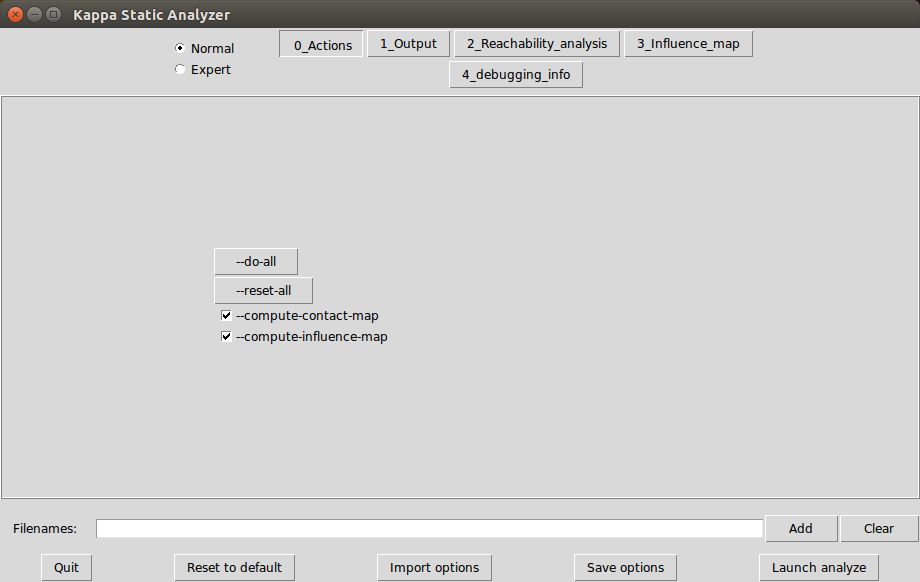
\includegraphics[width=12cm,natwidth=920pt,natheight=582pt]{img/kasa_0.png}
\caption{\KaSa~ graphical interface - sub-tab \texttt{0\_Actions}}
\label{fig:kasa:0}
\end{figure}

\subsection{The areas of interests}

There are five different areas of importance in the graphical interface:
\begin{enumerate}
\item On the top left of the window, a button allows for the selection between the Normal and the Expert mode (other modes may be available if activated at compilation).
In expert modes, more options are available in the graphical interface.
\item On the top center/right, some button allows for the selection of the tab. There are currently five sub-tabs available: \texttt{0\_Actions}, \texttt{1\_Output}, \texttt{2\_Reachability\_analysis}, \texttt{3\_Influence\_map}, \texttt{4\_debugging\_information}.
\item Center: The options of the selected sub-tab are displayed and can be tuned.

Contextual help is provided when the mouse is hovered over an element.

The interface will store the options that are checked or filled and the order in which they have been selected.
When launched, the analysis interprets these options in the order they have been entered.

Some options appear in several sub-tabs. They denote the same option and share the same value.

\item File selector: The file selector can be used to upload as many kappa files as desired. The button '\texttt{Clear}' can be used to reset the selection of files.
\item Bottom: Some buttons are available. The button '\texttt{Quit}' can be used to leave the interface. The button '\texttt{Reset to default}' tune all the options to their default value. The button '\texttt{Import options}' can be used to restore the value of the options as saved during a previous session of the graphical interfaces. The button '\texttt{Save options}' can be used to save the value of the options for a further session. The button '\texttt{Launch analyze}' launch \KaSa\ with the current options.

Importantly, options are saved automatically under various occasions. Thus, it is possible to restore the value of the options
before the last reset, before the last quit, or before the last analysis.
\end{enumerate}

\subsection{The sub-tab \texttt{0\_Actions}}

The sub-tab \texttt{0\_Actions} (see Fig.~\ref{fig:kasa:0}) contains the main actions which can be performed.

\begin{itemize}
\item The button \texttt{--do-all} activates all the functionalities.
\item The button \texttt{--reset-all} inactivates all the functionalities.
\item The option \texttt{--compute-contact-map} can be used to (des)activate the computation of the contact map.
\item The option \texttt{--compute-influence-map} can be used to (des)activate the computation of the influence map.
\item The option \texttt{--compute-reachability-analysis} can be used to (des)activate the computation of the reachability analysis.
\item The option \texttt{--compute-local-traces} can be used to (des)activate the computation of the trace analysis.
\end{itemize}

\subsection{The sub-tab \texttt{1\_Output}}

\begin{figure}[htbp]
\centering
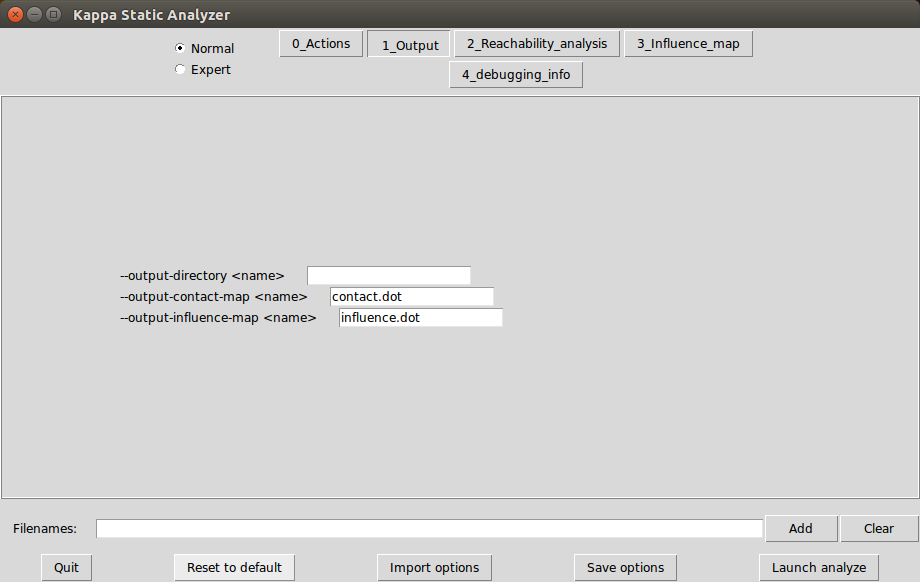
\includegraphics[width=12cm,natwidth=920pt,natheight=582pt]{img/kasa_1.png}
\caption{\KaSa~ graphical interface - sub-tab \texttt{1\_output}}
\label{fig:kasa:1}
\end{figure}


The sub-tab \texttt{1\_Ouput} (see Fig.~\ref{fig:kasa:1}) contains the names of the output files.

\begin{itemize}
\item The field \texttt{--output-directory} can be used to set the repository where output file are written. \KaSa~will create this repository, if it does not exist.
\item The field \texttt{--output-contact-map-directory} can be used to set the reporitory where the output file for the contact map is written, if a contact map is requested. \KaSa~will create this repository, if it does not exist.
\item The field \texttt{--output-influence-map-directory} can be used to set the reporitory where the output file for the influence map is written, if an influence map is requested. \KaSa~will create this repository, if it does not exist.
\item The field \texttt{--output-local-traces-directory} can be used to set the reporitory where the output file for the result of trace analysis is written, if this analysis is requested. \KaSa~will create this repository, if it does not exist.
\item The field \texttt{--output-contact-map} contains the name of the file for the contact map.
\item The field \texttt{--output-influence-map} contains the name of the file for the influence map.
\end{itemize}

When a file already exists, it is overwritten without any warning.

\section{Reachability analysis}

\begin{figure}[htbp]
\centering
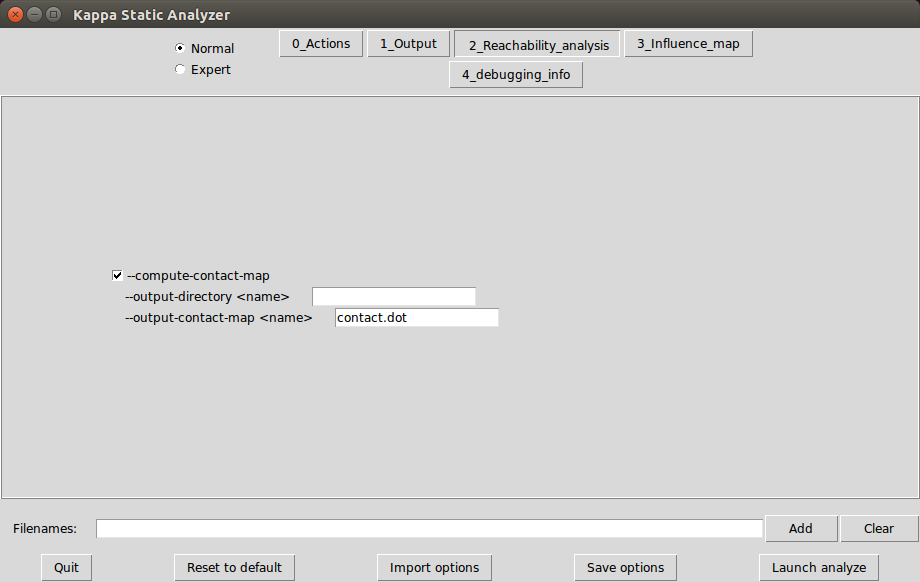
\includegraphics[width=12cm,natwidth=920pt,natheight=582pt]{img/kasa_2.png}
\caption{\KaSa~ graphical interface - sub-tab \texttt{2\_Reachability\_analysis}}
\label{fig:kasa:2}
\end{figure}

Reachability analysis aimed at detecting statically properties about the bio-molecular species that can be formed in a model.
Knowing whether, or not, a given bio-molecular species, can be formed in a model is an undecidable problem \cite{Kreyssig}. Thus, our analysis is approximate. Indeed, it computes an over-approximation of the set of the bio-molecular species that can be reached from the initial state of the model, by applying an unbounded number of computation steps. As formalized in \cite{DanosEtAl-VMCAI08}, the abstraction consists in:
\begin{enumerate}
\item firstly, ignoring the number of occurrences of bio-molecular species (we assume that whenever a bio-molecular species can be formed, then it can be formed as many time as it could be necessary),
\item secondly, abstracting a bio-molecular species by the set of its local views (that is to say that we focus on the relationships between the states of the sites within agents, but we abstract away any relationships between different agents within a bio-molecular species).
\end{enumerate}

As an example, we consider the following model:
\begin{lstlisting}[language=kappa]
'A.p'   A(x~u,y) -> A(x~p,y)
'dimer' A(x~p,y),A(x~p,y) -> A(x~p,y!1),A(x~p,y!1)
'dead'  A(x~u,y!_) -> A(x~q,y)

%init: 1 A(x~u,y~u)
\end{lstlisting}

Typing the following instruction:
\begin{verbatim}
KaSa reachability.ka --reset-all --compute-reachability-analysis
\end{verbatim}

will perform the reachability analysis on the model \texttt{reachability.ka}.


The result (eg.~see Fig.~\ref{fig:reachability_low}) is displayed in the standard output, and it is made of three parts:
\begin{itemize}
\item \textbf{Detection of dead rules.} A rule is called dead, if there is no trace starting from the initial state in which this rule is applied. The analysis reports the list of the rules it has detected to be dead. Due to the over-approximation, it may happen that a dead rule is not discovered by the analysis. Yet, any rule that is reported as dead, is dead indeed.

\item \textbf{Relational properties.} The analysis detects some relationships among the states of the sites of each agent. Simple properties are reported in natural languages. More complex properties are reported in extension, by enumerating the states that these site can take simultaneously within a given instance of an agent. Due to the over-approximation of the analysis, the analysis may fail in discovering a relationship. But each relationship that is found by the analysis, is satisfied.

\item \textbf{Non-relational properties.} The analysis detects for each kind of site, the set of states this site can take. This set is described in natural language. Due to the over-approximation, the analysis reports a super-set of the set of the potential states. Yet, we are sure that a given site only take states within this set.
\end{itemize}

\begin{figure}[t]
\input{generated_img/LOG_mute.txt}
\caption{Reachability analysis of the model \texttt{reachbility.ka} with verbosity level ``Mute''.}
\label{fig:reachability_mute}
\end{figure}
\begin{figure}[p]
\input{generated_img/LOG_low.txt}
\caption{Reachability analysis of the model \texttt{reachbility.ka} with verbosity level ``Low''.}
\label{fig:reachability_low}
\end{figure}
\begin{figure}[p]
\input{generated_img/LOG_medium_KO.txt}
\caption{Reachability analysis: one rule that cannot be applied yet, according to the bio-molecular species already constructed.}
\label{fig:reachability_medium_ko}
\end{figure}

\begin{figure}[p]
\input{generated_img/LOG_medium_OK.txt}
\caption{Reachability analysis: one rule successfully applied}
\label{fig:reachability_medium_ok}
\end{figure}

\begin{figure}[p]
\input{generated_img/LOG_high_init.txt}
\caption{Reachability analysis: extensional description of initial states.}
\label{fig:reachability_high_init}
\end{figure}

\begin{figure}[p]
\input{generated_img/LOG_high_rule.txt}
\caption{Reachability analysis: extensional description of the new views created when applying a rule.}
\label{fig:reachability_high_rule}
\end{figure}

\begin{figure}[p]
\input{generated_img/LOG_full.txt}
\caption{Reachability analysis: discovering new views force the analysis to apply some rules again, until reaching a fix-point.}
\label{fig:reachability_full}
\end{figure}

The option \verb?--use-natural-language? can be used to switch on/off the translation of properties in natural language: when the option is disabled, each relationship is described in extension.

It is possible to get more details about the computation of the analysis by tuning the verbosity level of the view analysis:
\begin{itemize}
\item With the option \verb?--use-natural-language Mute?, nothing is displayed. Even the result of the analysis is omitted (eg.~see Fig.~\ref{fig:reachability_mute}).




\item With the option \verb?--use-natural-language Low?, only the result of the analysis is displayed (eg.~see Fig.~\ref{fig:reachability_low}).



\item With the option \verb?--use-natural-language Medium?, the analysis also describes which rules are applied and in which order.

When trying to apply a rule, the analysis may detect that the rule cannot be applied yet because the precondition is not satisfied at the current state of the iteration (eg.~see Fig.~\ref{fig:reachability_medium_ko}). Otherwise, the analysis can apply the rule and update the state of the iteration accordingly (eg.~see Fig.~\ref{fig:reachability_medium_ok}).



\item With the option \verb?--use-natural-language High?, the analysis also describes which views are discovered.

In particular, at the beginning of the iteration, the analysis prompts the views that occur in initial state (eg.~see Fig.~\ref{fig:reachability_high_init}). Then, each time a rule is applied successfully, the analysis shows which new views have been discovered (eg.~see Fig.~\ref{fig:reachability_high_rule}).



\item When new views are discovered, then, it is necessary to apply again any rule that may operate over these views. With the option \verb?--use-natural-language Full?, the analysis also describes which rules are awaken by the discovery of a new view (see Fig.~\ref{fig:reachability_full}).



\end{itemize}

\section{Local traces}
\label{sec:local-traces}

This section is under construction.

\begin{figure}[htbp]
\centering
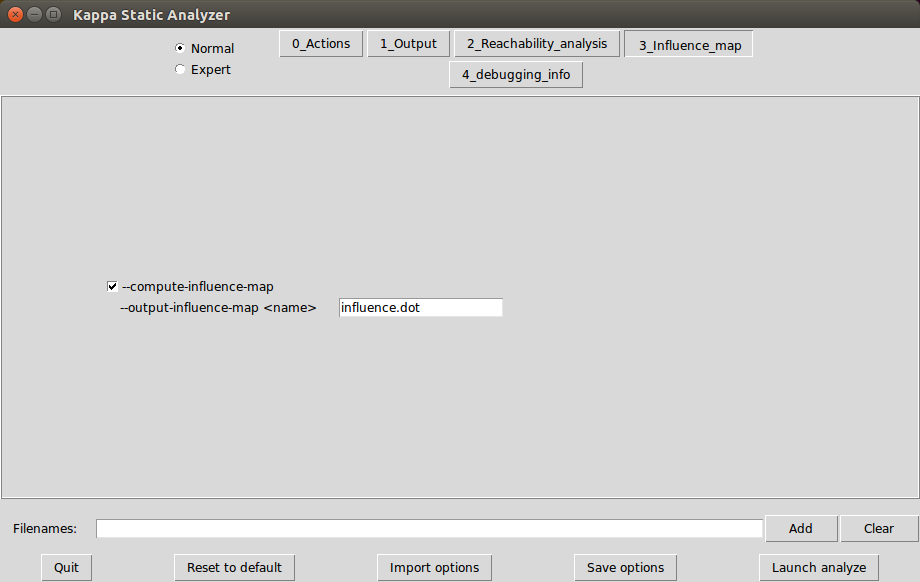
\includegraphics[width=12cm,natwidth=920pt,natheight=582pt]{img/kasa_3.png}
\caption{\KaSa~ graphical interface - sub-tab \texttt{3\_Trace\_analysis}}
\label{fig:kasa:3}
\end{figure}

Trace analysis is a refinement of reachability analysis that additionaly explains how one agent can go from a given view to another one, following a path that we call a local trace.
Thus the set of the local traces for a given agent can be described as a transition system among the views for a given agent: in this transition system, the nodes are local views; introduction arrows correspond to either initial states, or creation rules; transitions denote a potential conformation change of an agent, from one local views to another one, due to the application of a given rule.

We consider the following example:
\begin{lstlisting}[language=kappa]
  %init: 1 P()
  %init: 1 K()

  'a1+' P(a1~u) -> P(a1~p) @1
  'b1+' P(a1~p,b1~u) -> P(a1~p,b1~p) @1
  'a1-' P(a1~p,b1~u) -> P(a1~u,b1~u) @1
  'b1-' P(b1~p,g) -> P(b1~u,g) @1
  'a2+' P(tab:siga2~u) -> P(a2~p) @1
  'a2-' P(a2~p,g) -> P(a2~u,g) @1
  'b2+' P(a2~p,b2~u) -> P(a2~p,b2~p) @1
  'b2-' P(b2~p,g) -> P(b2~u,g) @1
  'P.K' P(a1~p,a2~p,b1~p,b2~p,g),K(x) -> P(a1~p,a2~p,b1~p,b2~p,g!1),K(x!1) @1
  'P/K' P(a1~p,a2~p,b1~p,b2~p,g!1),K(x!1) -> P(a1~p,a2~p,b1~p,b2~p,g),K(x) @1
\end{lstlisting}

Typing the following instruction:

\begin{verbatim}
KaSa protein2x2.ka --reset-all --compute-local-traces
\end{verbatim}

will perform the trace analysis on the model \texttt{protein2x2ka}, and produce
two dot format files \texttt{Agent\_trace\_K\_x\string^.dot} and \texttt{Agent\_trace.P.a1\_.a2\_.b1\_.b2\_.g\string^.dot}. The  output repository can be changed thanks to the command line options \texttt{--output-directory} and \texttt{--output-local-trace-directory}. Moreover, file names is made of the prefix \texttt{Agent\_trace}, followed by  the kind of protein and the list of the sites of interest (the symbol `\texttt{\string^}' denotes a binding state, and the symbol `\texttt{\_}' an internal state).

The transition system that describes the local traces for the agents of kind $P$ is descrided in Figure \ref{fig:trace-raw}. We notice that the nodes of this transition system are labelled with the states of the sites of $P$. The internal state of a site $x$ is denoted as $x{\sim}u$ (meaning that the site $x$ has state $u$, whereas the binding state of a site $x$ is denoted as $x!\textit{free}$, when the site is free, and as $x!K@x$ when the site $x$ is bound to the site $x$ of a given agent of kind $K$.

\begin{figure}[htbp]
\centering
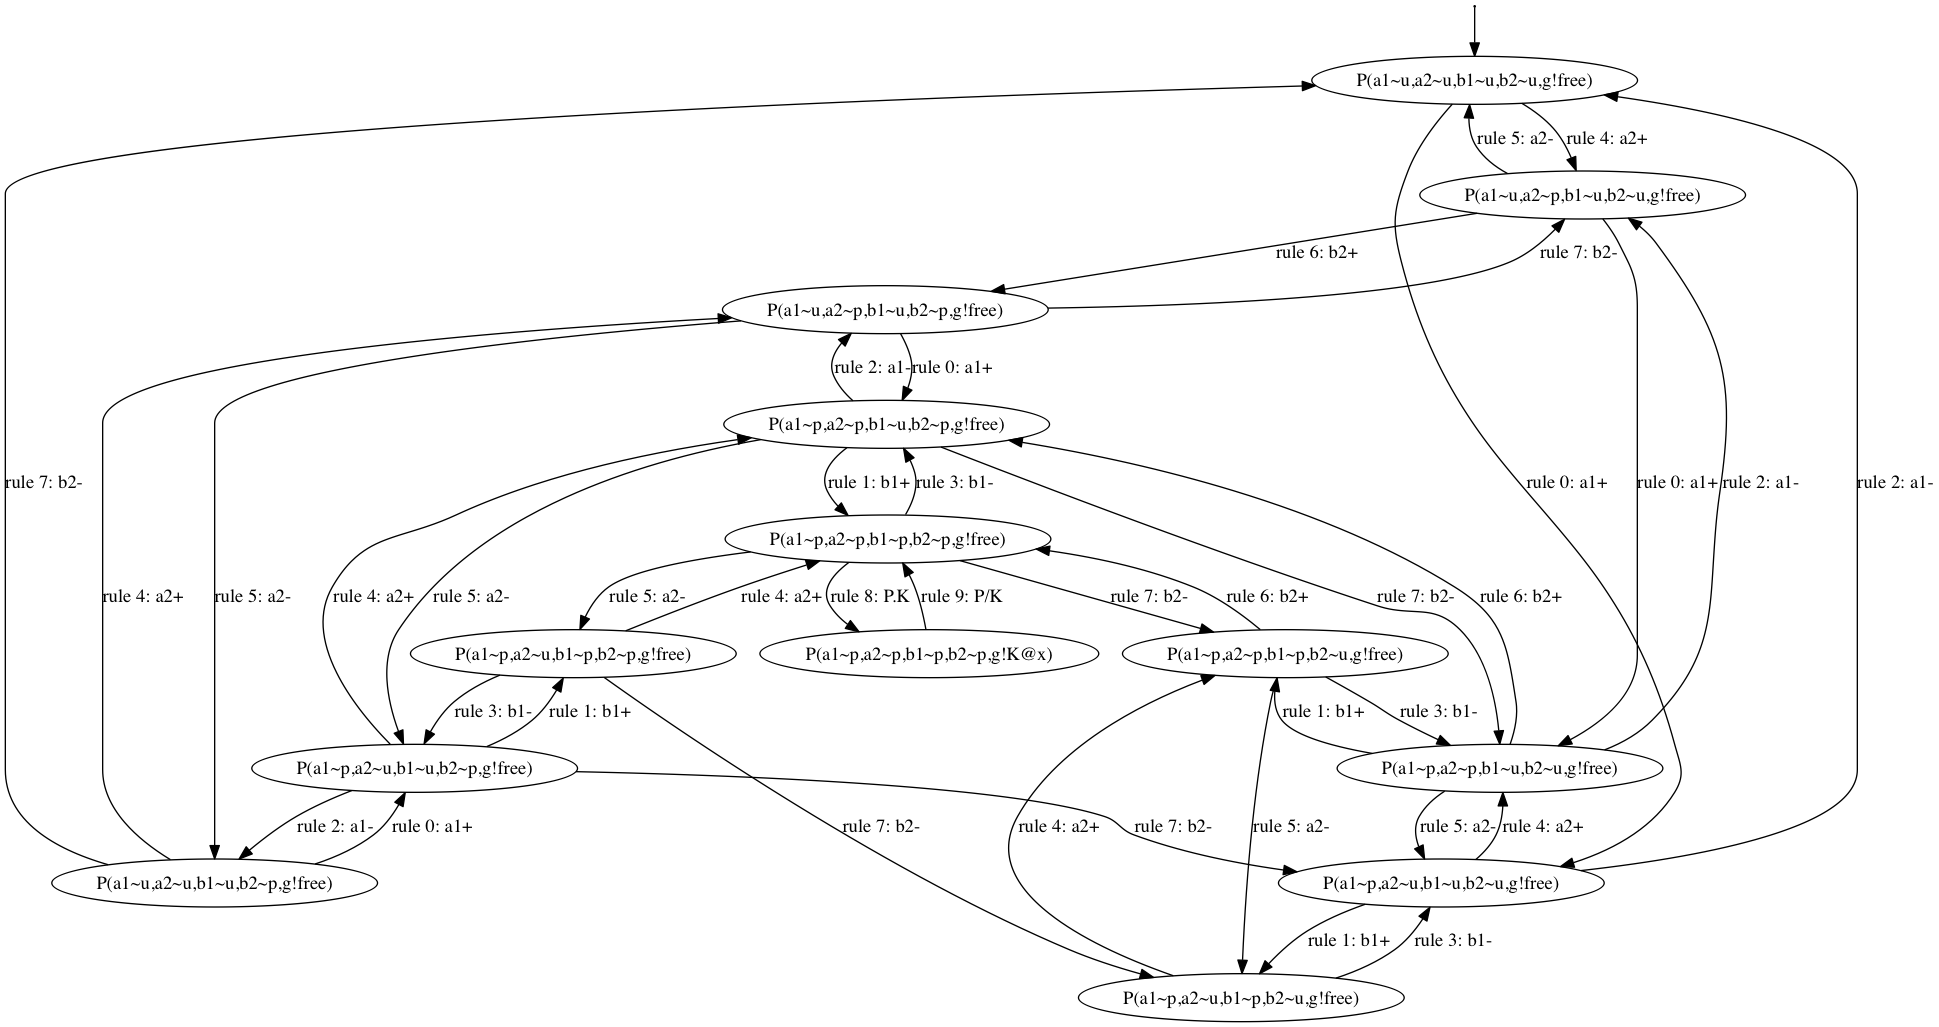
\includegraphics[width=10cm,natwidth=1939pt,natheight=1027pt]{generated_img/trace_raw.png}
\caption{Local traces for the \ttt{protein2x2.ka} model defined in Section~\ref{sec:local-traces}}
\label{fig:trace-raw}
\end{figure}

We notice that the transition system that is given in Fig.~\ref{fig:trace-raw}  contains too many nodes. We can coarse-grain this transition system thanks to the following option:
\begin{center}
\texttt{--use-macrotransitions-in-local-traces}.
\end{center}
Typing the following instruction:

\begin{verbatim}
KaSa protein2x2.ka --reset-all --compute-local-traces
                   --use-macrotransitions-in-local-traces
\end{verbatim}

will perform the trace analysis on the model \texttt{protein2x2ka}, and produce
two dot format files \texttt{Agent\_trace\_K\_x\string^.dot} and \texttt{Agent\_trace.P.a1\_.a2\_.b1\_.b2\_.g\string^.dot}. The name of the output repository can be changed thanks to the command line options \texttt{--output-directory} and \texttt{--output-local-trace-directory}.
This time, the files describe a coarse-graining of the corresponding transition systems.

For instance, the coarse-grained transition system for the local traces of the proteins of kind $P$, is given in Figure~\ref{fig:trace-macro}.  This  coarse-grained transition system is a compact implicit encoding of the transition system in Figure~\ref{fig:trace-raw}. It is obtained by exploiting the fact that locally, the behavior of the pair of states $a_1$ and $b_1$ is independent from the behavior of the pair of states $a_2$ and $b_2$, until these four sites are phosphorylated, so that the site $g$ can get bound.


More formally, in that transition system, some states are microstates (in a microstate, the state of each site is documented); some others are macrostates: (in a macrostate, the states of only a subset of site is documented).
Thus a macrostate $v^{\sharp}$ can be seen intensionally as a part  of a local view, but also extensionnaly as the set $\gamma(v^{\sharp})$ of the local views they are a subpart of. A microstate $v$ can be described by any sequence $(v_i^{\sharp})$ of macrostates prodiding that the intersection $\bigcap \gamma(v^{\sharp}_i)$ of the extensional denotation $\gamma(v^{\sharp}_i)$ of these macrostates $v^{\sharp}_i$, is equal to the singleton $\{v\}$;
moreover a transition between two microstates $v$ and $v'$ can be described by any transition between one macro state $v^{\sharp}$ and another one $v'{}^{\sharp}$, provided that there exists a sequence of macrostate $(v^{\sharp}_i)$ such that the sequence $(v^{\sharp},(v^{\sharp}_i))$ denotes the microstate $v$ and the sequence $(v'{}^{\sharp},(v^{\sharp}_i))$ denotes the microstate $v'$.

\begin{figure}[htbp]
\centering
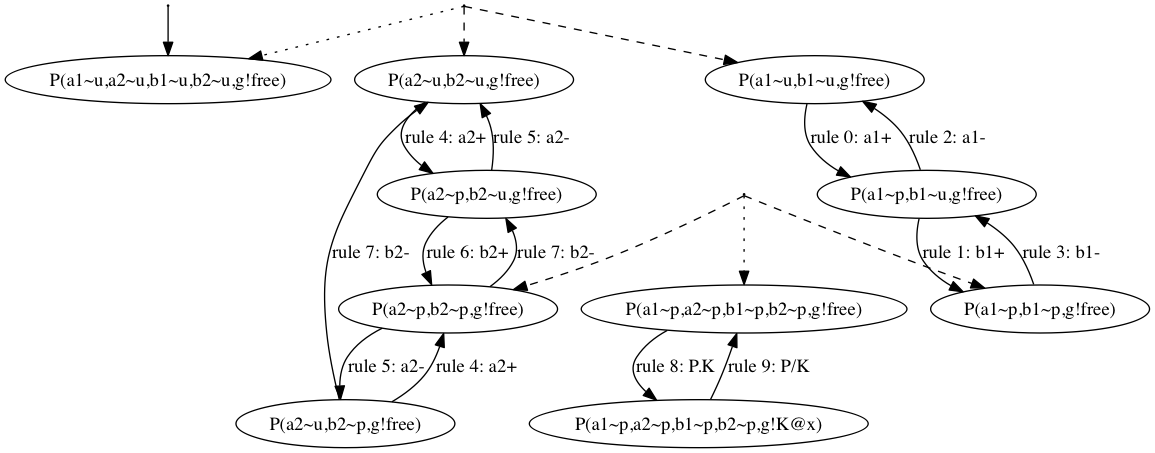
\includegraphics[width=10cm,natwidth=1155pt,natheight=453pt]{generated_img/trace_macro.png}
\caption{Local traces for the \ttt{protein2x2.ka} model defined in Section~\ref{sec:local-traces}}
\label{fig:trace-macro}
\end{figure}

Such coarse-grained transition system can be geometrically interpreted as a simplicial complex \cite{DBLP:conf/concur/FajstrupGR98}.

As a microstate could be decomposed into several sequences of macrostates (including the trivial sequence containing only the microstate itself), the system may jump spontaneously (by using a $\varepsilon$ transition) from one representation to another representation. This corresponds to the intersection between several simplexes in the corresponding simplificial complex.

Although the semantics of a coarse-grainged transition system is fully defined  by its labelled transitions, it is useful to annotate the graph by some information about the relation between the denotation of each macrostate. By default, we use hypertlinks to relate each macrostate $v$ (including each microstate)
 to the set of its immediate subparts $v'$. In such a hyperlink, $v$ is connected via a dotted arrow, whereas each immediate subpart is connected via a dashed arrow.

 More options are available in expert mode, but they are not documented yet.

\section{Contact map}

The contact map of a model is an object that may help modelers checking the consistency of the rule set they use. The contact map is \emph{statically} computed and does not depend on kinetic rates nor initial conditions.


Typing the following instruction:

\texttt{KaSa abc.ka --reset-all --compute-contact-map}

will produce a dot format file named \texttt{contact.dot}.
The name of the output file and the directory can be changed to the command line options \texttt{--output-contact-map} and \texttt{--output-directory}.
The directory is assumed to exist. The file will be overwritten if it exists. All the options related to the computation of the contact map can be accessed on the
sub-tab \texttt{3\_Reachability\_analysis} of the graphical interface (see Fig.~\ref{fig:kasa:3}).




The contact map summarises the different types of agent, their interface and the potential binding between sites. It is an over approximation, thus if the contact map indicates a potential bond, it does not mean that it is always possible to reach a state in which two sites of these kinds are bound, but if the contact map indicates no bond between two sites, it means that it is NOT possible to reach a state in which two sites of these kinds are bound together.


The contact map for the \ttt{abc.ka} model  defined in Chapter~\ref{chap:abc} is given in Figure~\ref{fig:abc-contact}. On this map, we notice that there are three kinds of agent, namely $A$, $B$, and $C$.
Agents of kind $A$ have two sites $x$ and $c$, that bear no internal state (they appear in yellow only), agents of kind $B$ have one site $x$, that bears no internal state (they appear in yellow only), and agents of kind $C$ have two sites $x_1$ and $x_2$ with both a binding state and an internal state (they appear both in yellow and in green). We notice that when a site can bear both an internal state and a binding state, they are considered as two different sites in the contact map. Additionally, the contact map indicates that sites $x$ of the agents of kind $A$ can be bound to the site $x$ of an agent of kind $B$ and that sites $c$ of the agents of kind $A$ can be bound to the agents of kind $C$ either on the site $x_1$, or on the site $x_2$.

\begin{figure}[htbp]
\centering
\includegraphics[width=8cm,natwidth=920pt,natheight=582pt]{generated_img/abc_contact.png}
\caption{Contact Map for the \ttt{abc.ka} model defined in Chapter~\ref{chap:abc}}
\label{fig:abc-contact}
\end{figure}



\section{Influence map}

The influence map of a model is an object that may help modelers checking the consistency of the rule set they use.

Typing the following instruction:

\texttt{KaSa abc.ka --reset-all --compute-influence-map}

will produce a dot format file named \texttt{influence.dot}.
The name of the output file and the directory can be changed to the command line options \texttt{--output-influence-map} and \texttt{--output-directory}.
The directory is assumed to exist. The file will be overwritten if it exists.  All the options related to the computation of the influence map can be accessed on the sub-tab \texttt{4\_Influence\_map} of the graphical interface (see Fig.~\ref{fig:kasa:4}).

\begin{figure}[htbp]
\centering
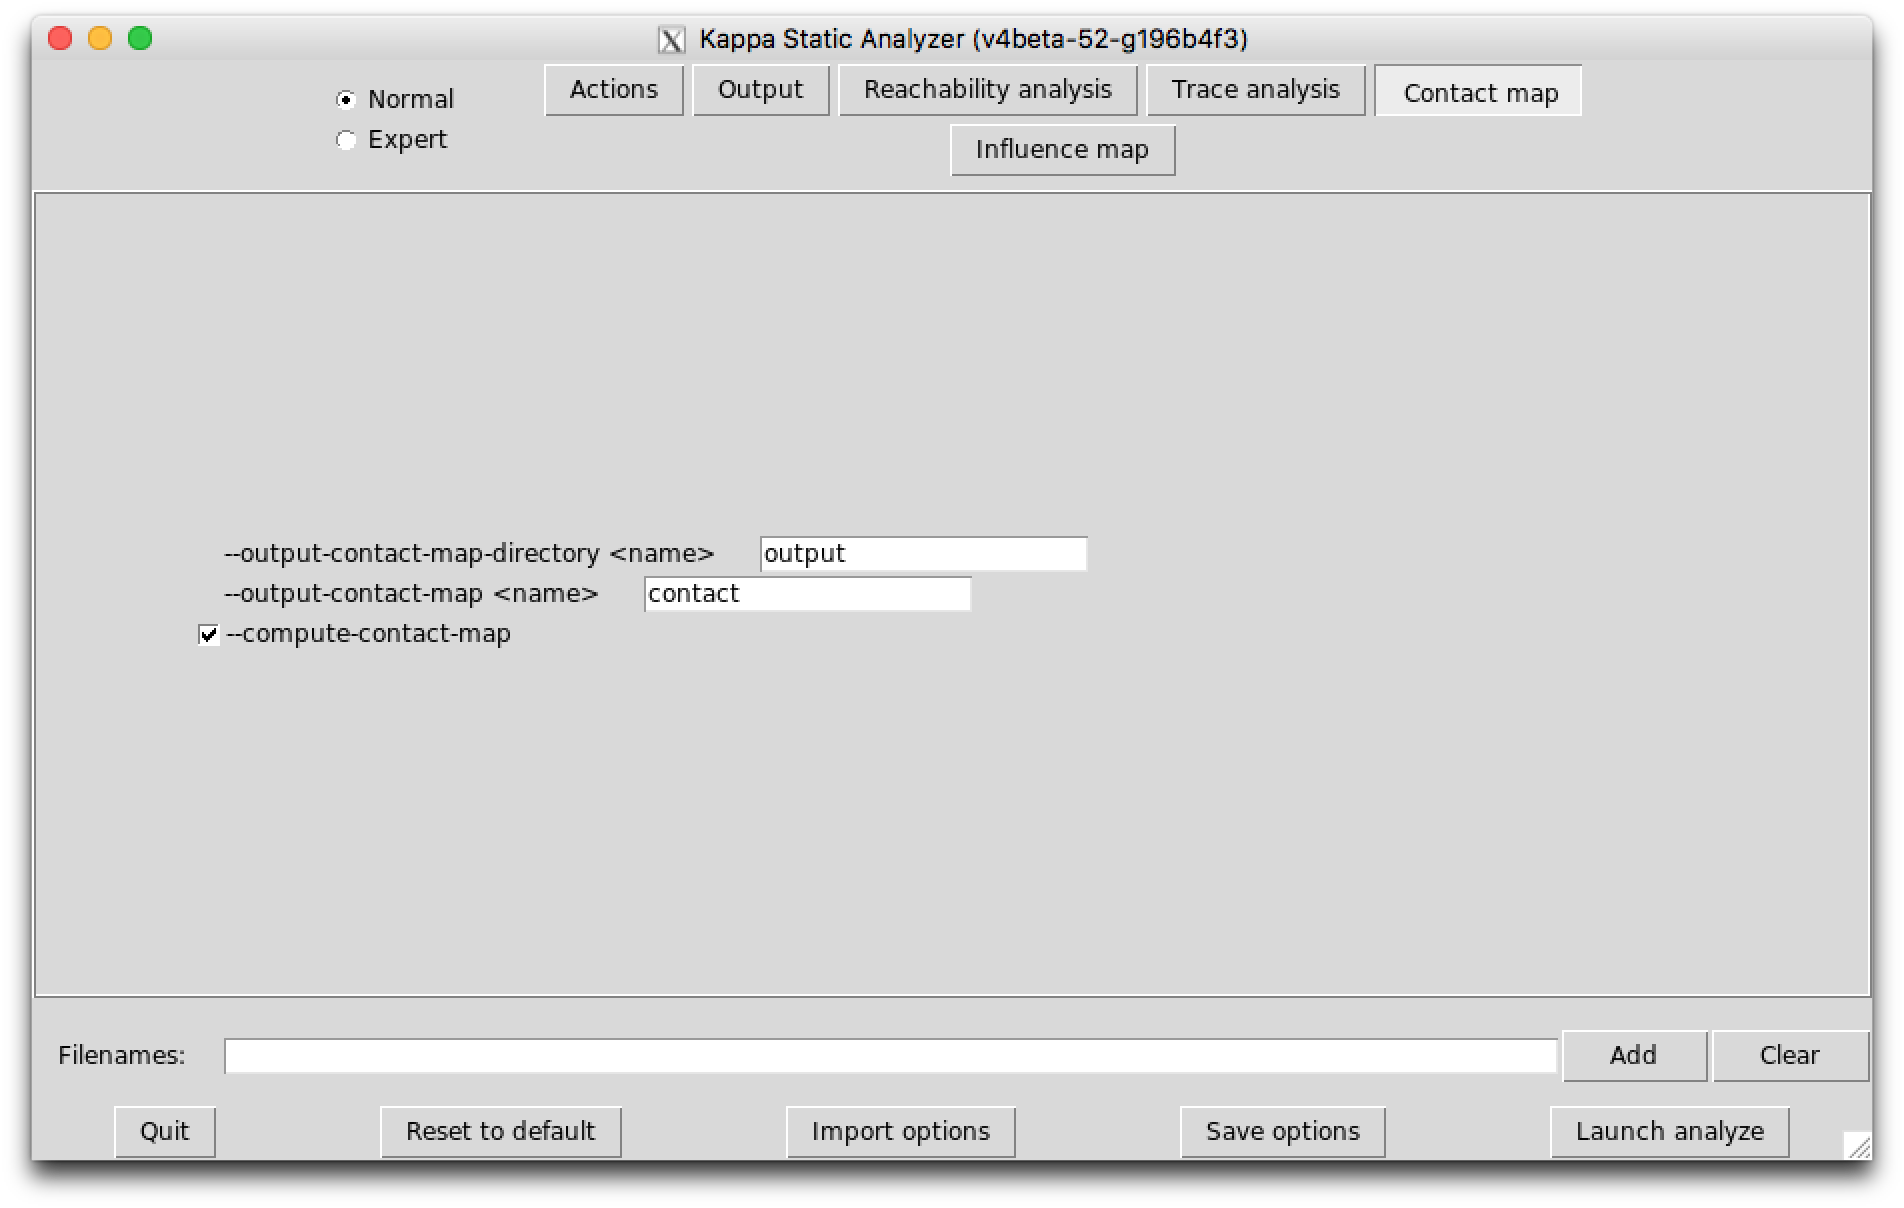
\includegraphics[width=12cm,natwidth=920pt,natheight=582pt]{img/kasa_4.png}
\caption{\KaSa~ graphical interface - sub-tab \texttt{4\_Influence\_map}}
\label{fig:kasa:4}
\end{figure}

Unlike the flux map, the influence map is \emph{statically} computed and does not depend on kinetic rates nor initial conditions. It describes how rules may potentially influence each other during a simulation. \KaSa~will produce a dot format file containing the influence relation over all rules and observables of the model. The produced graph visualised using a circular rendering\footnote{One may use for instance the \ttt{circo} program that is part of the \textit{graphviz} suite.} is given in Figure~\ref{fig:kasa-abc-im}. Observables are represented as circular nodes and rules as rectangular nodes. The labels of the nodes are either the label of the rule or of the observable (if available), otherwise it is made of a unique identifier allocated by \KaSa~followed by the kappa definition of the rule/observable.
Edges are decorated with the list of embeddings (separated by a semi-colon) allowing the identification of agents in both rules{\textquotesingle}s right hand sides/left hand sides.
More precisely, for positive influences,  the notation $[i\rar j]$ denotes a pair of embeddings from the agent number $i$ of the origin{\textquotesingle}s right hand side and from the agent number $j$ of the target{\textquotesingle}s left hand side and the notation $[i\star \rar j]$ denotes a pair of embeddings from an agent attached to the agent number $i$  of the origin{\textquotesingle}s left hand side, which have been freed by side effect  and   from the agent number $j$ of the target{\textquotesingle}s left hand side; for negative influences,  the notation $[i\rar j]$ denotes a pair of embeddings from the agent number $i$ of the origin{\textquotesingle}s left hand side and from the agent number $j$ of the target{\textquotesingle}s left hand side and the notation $[i\star \rar j]$ denotes a pair of embeddings from an agent attached to the agent number $i$  of the origin{\textquotesingle}s left hand side, which have been freed by side effect  and   from the agent number $j$ of the target{\textquotesingle}s left hand side;
 Observables have no influence, but they can be influenced by rules, if the rule can increase or decrease their value.


\begin{figure}[htbp] %  figure placement: here, top, bottom, or page
   \centering
   \includegraphics[width=15cm]{generated_img/abc_influence.png}
   \caption{The influence map of the \ttt{abc.ka} model defined in Chapter~\ref{chap:abc}. Edge labels denote embeddings with the convention that
the notation $[i\rar j]$, in a positive influence, denotes a pair of embeddings from the agent number $i$ of the origin{\textquotesingle}s right hand side and from the agent number $j$ of the target{\textquotesingle}s left hand side;
the notation $[i\rar j]$, in negative influence,  denotes a pair of embeddings from the agent number $i$ of the origin{\textquotesingle}s left hand side and from the agent number $j$ of the target{\textquotesingle}s left hand side;
the notation $[i\star \rar j]$, whatever the influence is positive of negative,  denotes a pair of embeddings from an agent attached to the agent number $i$  of the origin{\textquotesingle}s left hand side, which have been freed by side effect  and   from the agent number $j$ of the target{\textquotesingle}s left hand side. }
   \label{fig:kasa-abc-im}
\end{figure}

More formally, consider the rules $r:L\rar R$ and $s:L'\rar R'$. One wishes to know whether it is possible that the application of rule $r$ over a graph $G$ creates a new instance of rule $s$ (which is called a positive influence and that is described by green arrows in the influence map), or destroy a previous instance of rule $s$ (which is called negative influence and that is described by red arrows in the influence map).
In Fig.~\ref{fig:imbis}, we illustrate the construction of positive influences due to overlap of the left hand side of a rule and the right hand side of another rule on some sites that are modified by the former one.

\begin{figure}[htbp] %  figure placement: here, top, bottom, or page
   \centering
\includegraphics[width=8cm,natwidth=1462pt,natheight=756pt]{img/im.png}
   \caption{Computation of the influence of the top rule on the rule below: the right hand side of the first rules embeds in a common term with the left hand side of the second rule. It results that the first rule has a positive influence on the second.}
   \label{fig:imbis}
\end{figure}

The current implementation has the following limitations:
\begin{itemize}
\item Currently, only observables that are defined as patterns are taken into account.
\item Not atomic observables which are defined as algebraic expressions are not taken into account yet. The observables are ignored.
\item The influence map does not take into account indirect influences due to perturbations (which could arises when the application of a rule triggers a perturbation which would create some agents or increase/decrease the value of some variables).
\item Token are not taken into yet. They are currently ignored.
\item Positive/negative influence of time is not taken into account either.
\end{itemize}

Lastly, KaSa\ computes an over-approximation of the influence map. They may show an influence despite the fact that there can be no actual one. But if it shows no influence it means that either there are NO such influence, or that we are in a case that is not covered yet as itemised previously.

\chapter{Frequently asked questions}
\section*{Simulation hangs after a while}
If the progress bar seems stalled, it does not necessarily mean that the simulation is blocked. In particular when a simulation is triggered with a \emph{time} limit (\ttt{-t} option of the command line) it might only indicate that the bio clock is stalled while computation events still occur. Recall that the average (bio) time one has to wait in order to apply a rule is $1/A$, where $A$ is the sum of all the rule activities (which is equal to the number of instances that a rule has, times its kinetic rate). Whenever the number of occurrences of a rule grows too fast (if new agents are created during the simulation for instance), or if the kinetic rate of a rule is defined by a function that grows rapidly, the average time increment might tend to 0 and if it remains so for a while, it will block the progress bar whose advance is proportional to the bio time \ttt{[T]}.

In order to make sure that \KaSim~is not incorrectly blocked you may wish to plot the event clock against time clock using the observable \ttt{\%obs: {\textquotesingle}events{\textquotesingle} [E]} or run the simulation using an event limit (\ttt{-e} option of the command line) instead of a time limit.

\section*{What do null events mean, why do I have any?}

Null events\index{null event} is a way for \KaSim~to compensate for some over approximation it is doing, in order deal with large simulations more efficiently. They usually do not impact significantly the performances of the simulator, unless the model contains rules using the special notation to deal with ambiguous molecularity (see Section~\ref{sec:ambiguous}). With pure Kappa rules, the ratio $r$ of null event over productive ones (that you can track using the observable \ttt{\%obs: {\textquotesingle}r{\textquotesingle}  [E-]/[E]}) should tend to 0 when models have a lot of agents.

\section*{No data points are generated}
Make sure you have \ttt{\%obs} or \ttt{\%plot} instructions in your KF\index{kappa file}. Also make sure to use the \ttt{-p} option in the command line to tell KaSim how many points you wish to have on your curves.

\section*{Too many instances of an observable}
The value of a kappa expression $E$  is equal to the number of embeddings\index{embedding} it has in the current mixture\index{mixture} $M$. Embeddings are maps from agents in $E$  to agents in $M$. If $E$ has symmetries then every permutation of $E$ will be counted as a new embedding. For instance let $E=$\ttt{A(x!1),A(x!1)}  and let $M=$\ttt{A(x!1,y\intstate p),A(x!1,y\intstate u)}.
\KaSim~will count two instances of $E$ in $M$: the one mapping the first \ttt{A} of $E$ to the first \ttt{A} of $M$ and the one mapping the first \ttt{A} of $E$ to the second \ttt{A} of $M$.

\section*{The computed influence map is incorrect, it misses some activation or has too much of them}
The influence map\index{influence map} computed by \KaSim~contains relations that are computed on side effect free rules only. It is likely that a missing activation is due to a side effect that is not taken into account. If the influence map shows an activation between rule $r$ and $s$ that is never possible with a given model, just remember that activation computation implies that \emph{there exists} a context in which applying rule $r$ will create a new instance of rule $s$. This context might simply never be realized with the given rules or initial conditions.

\section*{Value \ttt{nan} in the data file\index{data file} at the end of the simulation}
The value \ttt{nan} means "Not a Number". It is generated when a plotted variable is infinite. Make sure this variable is not divided by zero at some point.

\bibliographystyle{plain}
\bibliography{fmb,concur,static_analyses}

\printindex

\end{document}
%%% Local Variables:
%%% ispell-local-dictionary: "british"
%%% End:
